% !TeX spellcheck = en_US
% !TeX encoding = UTF-8
% !TeX program = pdflatex

%\documentclass[11pt,a4paper,oneside]{report}             % Single-side
\documentclass[11pt,a4paper,twoside,openright]{report}  % Duplex

% thanks to http://tex.stackexchange.com/a/47579/71109
\usepackage{ifxetex}
\usepackage{ifluatex}
\newif\ifxetexorluatex % a new conditional starts as false
\ifnum 0\ifxetex 1\fi\ifluatex 1\fi>0
   \xetexorluatextrue
\fi

\ifxetexorluatex
  \usepackage{fontspec}
\else
  \usepackage[T1]{fontenc}
  \usepackage[utf8]{inputenc}
  \usepackage[lighttt]{lmodern}
\fi

\usepackage[english,magyar]{babel} % Alapértelmezés szerint utoljára definiált nyelv lesz aktív, de később külön beállítjuk az aktív nyelvet.

%\usepackage{cmap}
\usepackage{amsfonts,amsmath,amssymb} % Mathematical symbols.
%\usepackage[ruled,boxed,resetcount,linesnumbered]{algorithm2e} % For pseudocodes. % beware: this is not compatible with LuaLaTeX, see http://tex.stackexchange.com/questions/34814/lualatex-and-algorithm2e
\usepackage{booktabs} % For publication quality tables for LaTeX
\usepackage{graphicx}

%\usepackage{fancyhdr}
%\usepackage{lastpage}

\usepackage{anysize}
%\usepackage{sectsty}
\usepackage{setspace} % For setting line spacing

\usepackage[unicode]{hyperref} % For hyperlinks in the generated document.
\usepackage{xcolor}
\usepackage{listings} % For source code snippets.

\usepackage[amsmath,thmmarks]{ntheorem} % Theorem-like environments.

\usepackage[hang]{caption}

\singlespacing

\newcommand{\selecthungarian}{
	\selectlanguage{magyar}
	\setlength{\parindent}{2em}
	\setlength{\parskip}{0em}
	\frenchspacing
}

\newcommand{\selectenglish}{
	\selectlanguage{english}
	\setlength{\parindent}{0em}
	\setlength{\parskip}{0.5em}
	\nonfrenchspacing
	\renewcommand{\figureautorefname}{Figure}
	\renewcommand{\tableautorefname}{Table}
	\renewcommand{\partautorefname}{Part}
	\renewcommand{\chapterautorefname}{Chapter}
	\renewcommand{\sectionautorefname}{Section}
	\renewcommand{\subsectionautorefname}{Section}
	\renewcommand{\subsubsectionautorefname}{Section}
}


\usepackage{parskip,array,booktabs}
\usepackage{tikz}

%Additional
\usepackage{tabu}
\usepackage{todonotes}
\usepackage{multirow}
\usepackage{multicol}
\usepackage{enumitem}

\newcommand{\vikszerzoVezeteknev}{Ecsedi}
\newcommand{\vikszerzoKeresztnev}{Gergő}

\newcommand{\vikkonzulensAMegszolitas}{dr.~}
\newcommand{\vikkonzulensAVezeteknev}{Micskei}
\newcommand{\vikkonzulensAKeresztnev}{Zoltán}

\newcommand{\vikkonzulensBMegszolitas}{}
\newcommand{\vikkonzulensBVezeteknev}{}
\newcommand{\vikkonzulensBKeresztnev}{}

\newcommand{\vikkonzulensCMegszolitas}{}
\newcommand{\vikkonzulensCVezeteknev}{}
\newcommand{\vikkonzulensCKeresztnev}{}

\newcommand{\vikcim}{Developing a test environment for a railway demonstrator} % Cím
\newcommand{\viktanszek}{\bmemit} % Tanszék
\newcommand{\vikdoktipus}{\msc} % Dokumentum típusa (\bsc vagy \msc)
\newcommand{\vikmunkatipusat}{diplomaterv} % a "hallgató nyilatkozat" részhez: szakdolgozatot vagy diplomatervet

%--------------------------------------------------------------------------------------
% TDK-specifikus változók
%--------------------------------------------------------------------------------------
\newcommand{\tdkszerzoB}{Második Szerző} % Második szerző neve; hagyd üresen, ha egyedül í­rtad a TDK-t.
\newcommand{\tdkev}{2014} % A dolgozat írásának éve (pl. "2014") (Ez OTDK-nál eltérhet az aktuális évtől.)

% További adatok az OTDK címlaphoz (BME-s TDK-hoz nem kell kitölteni)
\newcommand{\tdkevfolyamA}{IV} % Első szerző évfolyama, római számmal (pl. IV).
\newcommand{\tdkevfolyamB}{III} % Második szerző évfolyama, római számmal (pl. III).
\newcommand{\tdkkonzulensbeosztasA}{egyetemi tanár} % Első konzulens beosztása (pl. egyetemi docens)
\newcommand{\tdkkonzulensbeosztasB}{doktorandusz} % Második konzulens beosztása (pl. egyetemi docens)

\newcommand{\szerzoMeta}{\vikszerzoVezeteknev{} \vikszerzoKeresztnev} % egy szerző esetén
%\newcommand{\szerzoMeta}{\vikszerzoVezeteknev{} \vikszerzoKeresztnev, \tdkszerzoB} % két szerző esetén

% Beállítások magyar nyelvű dolgozathoz
%%--------------------------------------------------------------------------------------
% Elnevezések
%--------------------------------------------------------------------------------------
\newcommand{\bme}{Budapesti Műszaki és Gazdaságtudományi Egyetem}
\newcommand{\vik}{Villamosmérnöki és Informatikai Kar}

\newcommand{\bmemit}{Méréstechnika és Információs Rendszerek Tanszék}

\newcommand{\keszitette}{Készítette}
\newcommand{\konzulens}{Konzulens}

\newcommand{\bsc}{Szakdolgozat}
\newcommand{\msc}{Diplomaterv}
\newcommand{\bsconlab}{BSc Önálló laboratórium}
\newcommand{\msconlabi}{MSc Önálló laboratórium 1.}
\newcommand{\msconlabii}{MSc Önálló laboratórium 2.}

\newcommand{\pelda}{Példa}
\newcommand{\definicio}{Definíció}
\newcommand{\tetel}{Tétel}

\newcommand{\bevezetes}{Bevezetés}
\newcommand{\koszonetnyilvanitas}{Köszönetnyilvánítás}
\newcommand{\fuggelek}{Függelék}

% Opcionálisan átnevezhető címek
%\addto\captionsmagyar{%
%\renewcommand{\listfigurename}{Saját ábrajegyzék cím}
%\renewcommand{\listtablename}{Saját táblázatjegyzék cím}
%\renewcommand{\bibname}{Saját irodalomjegyzék név}
%}

\newcommand{\szerzo}{\vikszerzoVezeteknev{} \vikszerzoKeresztnev}
\newcommand{\vikkonzulensA}{\vikkonzulensAMegszolitas\vikkonzulensAVezeteknev{} \vikkonzulensAKeresztnev}
\newcommand{\vikkonzulensB}{\vikkonzulensBMegszolitas\vikkonzulensBVezeteknev{} \vikkonzulensBKeresztnev}
\newcommand{\vikkonzulensC}{\vikkonzulensCMegszolitas\vikkonzulensCVezeteknev{} \vikkonzulensCKeresztnev}

\newcommand{\selectthesislanguage}{\selecthungarian}

\bibliographystyle{huplain}

\def\lstlistingname{lista}

\newcommand{\appendixnumber}{6}  % a fofejezet-szamlalo az angol ABC 6. betuje (F) lesz

% Settings for English documents
%--------------------------------------------------------------------------------------
% Elnevezések
%--------------------------------------------------------------------------------------
\newcommand{\bme}{Budapest University of Technology and Economics}
\newcommand{\vik}{Faculty of Electrical Engineering and Informatics}

\newcommand{\bmemit}{Department of Measurement and Information Systems}

\newcommand{\keszitette}{Author}
\newcommand{\konzulens}{Advisor}

\newcommand{\bsc}{Bachelor's Thesis}
\newcommand{\msc}{Master's Thesis}
\newcommand{\bsconlab}{BSc Project Laboratory}
\newcommand{\msconlabi}{MSc Project Laboratory 1}
\newcommand{\msconlabii}{MSc Project Laboratory 2}

\newcommand{\pelda}{Example}
\newcommand{\definicio}{Definition}
\newcommand{\tetel}{Theorem}

\newcommand{\bevezetes}{Introduction}
\newcommand{\koszonetnyilvanitas}{Acknowledgements}
\newcommand{\fuggelek}{Appendix}

% Optional custom titles
%\addto\captionsenglish{%
%\renewcommand*{\listfigurename}{Your list of figures title}
%\renewcommand*{\listtablename}{Your list of tables title}
%\renewcommand*{\bibname}{Your bibliography title}
%}

\newcommand{\szerzo}{\vikszerzoKeresztnev{} \vikszerzoVezeteknev}
\newcommand{\vikkonzulensA}{\vikkonzulensAMegszolitas\vikkonzulensAKeresztnev{} \vikkonzulensAVezeteknev}
\newcommand{\vikkonzulensB}{\vikkonzulensBMegszolitas\vikkonzulensBKeresztnev{} \vikkonzulensBVezeteknev}
\newcommand{\vikkonzulensC}{\vikkonzulensCMegszolitas\vikkonzulensCKeresztnev{} \vikkonzulensCVezeteknev}

\newcommand{\selectthesislanguage}{\selectenglish}

\bibliographystyle{plain}

\newcommand{\ie}{i.e.\@\xspace}
\newcommand{\Ie}{I.e.\@\xspace}
\newcommand{\eg}{e.g.\@\xspace}
\newcommand{\Eg}{E.g.\@\xspace}
\newcommand{\etal}{et al.\@\xspace}
\newcommand{\etc}{etc.\@\xspace}
\newcommand{\vs}{vs.\@\xspace}
\newcommand{\viz}{viz.\@\xspace} % videlicet
\newcommand{\cf}{cf.\@\xspace} % confer
\newcommand{\Cf}{Cf.\@\xspace}
\newcommand{\wrt}{w.r.t.\@\xspace} % with respect to

\newcommand{\appendixnumber}{1}  % a fofejezet-szamlalo az angol ABC 1. betuje (A) lesz


%--------------------------------------------------------------------------------------
% Page layout setup
%--------------------------------------------------------------------------------------
% we need to redefine the pagestyle plain
% another possibility is to use the body of this command without \fancypagestyle
% and use \pagestyle{fancy} but in that case the special pages
% (like the ToC, the References, and the Chapter pages)remain in plane style

\pagestyle{plain}
\marginsize{35mm}{25mm}{15mm}{15mm}

\setcounter{secnumdepth}{0}
%\sectionfont{\large\upshape\bfseries}
\setcounter{secnumdepth}{2}

\sloppy % Margón túllógó sorok tiltása.
\widowpenalty=10000 \clubpenalty=10000 %A fattyú- és árvasorok elkerülése
\def\hyph{-\penalty0\hskip0pt\relax} % Kötőjeles szavak elválasztásának engedélyezése


%--------------------------------------------------------------------------------------
% Setup hyperref package
%--------------------------------------------------------------------------------------
\hypersetup{
    % bookmarks=true,            % show bookmarks bar?
    unicode=true,              % non-Latin characters in Acrobat's bookmarks
    pdftitle={\vikcim},        % title
    pdfauthor={\szerzoMeta},    % author
    pdfsubject={\vikdoktipus}, % subject of the document
    pdfcreator={\szerzoMeta},   % creator of the document
    pdfproducer={},    % producer of the document
    pdfkeywords={},    % list of keywords (separate then by comma)
    pdfnewwindow=true,         % links in new window
    colorlinks=true,           % false: boxed links; true: colored links
    linkcolor=black,           % color of internal links
    citecolor=black,           % color of links to bibliography
    filecolor=black,           % color of file links
    urlcolor=black             % color of external links
}


%--------------------------------------------------------------------------------------
% Set up listings
%--------------------------------------------------------------------------------------
\definecolor{lightgray}{rgb}{0.95,0.95,0.95}
\lstset{
	basicstyle=\scriptsize\ttfamily, % print whole listing small
	keywordstyle=\color{black}\bfseries, % bold black keywords
	identifierstyle=, % nothing happens
	% default behavior: comments in italic, to change use
	% commentstyle=\color{green}, % for e.g. green comments
	stringstyle=\scriptsize,
	showstringspaces=false, % no special string spaces
	aboveskip=3pt,
	belowskip=3pt,
	backgroundcolor=\color{lightgray},
	columns=flexible,
	keepspaces=true,
	escapeinside={(*@}{@*)},
	captionpos=b,
	breaklines=true,
	frame=single,
	float=!ht,
	tabsize=2,
	literate=*
		{á}{{\'a}}1	{é}{{\'e}}1	{í}{{\'i}}1	{ó}{{\'o}}1	{ö}{{\"o}}1	{ő}{{\H{o}}}1	{ú}{{\'u}}1	{ü}{{\"u}}1	{ű}{{\H{u}}}1
		{Á}{{\'A}}1	{É}{{\'E}}1	{Í}{{\'I}}1	{Ó}{{\'O}}1	{Ö}{{\"O}}1	{Ő}{{\H{O}}}1	{Ú}{{\'U}}1	{Ü}{{\"U}}1	{Ű}{{\H{U}}}1
}


%--------------------------------------------------------------------------------------
% Set up theorem-like environments
%--------------------------------------------------------------------------------------
% Using ntheorem package -- see http://www.math.washington.edu/tex-archive/macros/latex/contrib/ntheorem/ntheorem.pdf

\theoremstyle{plain}
\theoremseparator{.}
\newtheorem{example}{\pelda}

\theoremseparator{.}
%\theoremprework{\bigskip\hrule\medskip}
%\theorempostwork{\hrule\bigskip}
\theorembodyfont{\upshape}
\theoremsymbol{{\large \ensuremath{\centerdot}}}
\newtheorem{definition}{\definicio}

\theoremseparator{.}
%\theoremprework{\bigskip\hrule\medskip}
%\theorempostwork{\hrule\bigskip}
\newtheorem{theorem}{\tetel}


%--------------------------------------------------------------------------------------
% Some new commands and declarations
%--------------------------------------------------------------------------------------
\newcommand{\code}[1]{{\upshape\ttfamily\scriptsize\indent #1}}
\newcommand{\doi}[1]{DOI: \href{http://dx.doi.org/\detokenize{#1}}{\raggedright{\texttt{\detokenize{#1}}}}} % A hivatkozások közt így könnyebb DOI-t megadni.

\DeclareMathOperator*{\argmax}{arg\,max}
%\DeclareMathOperator*[1]{\floor}{arg\,max}
\DeclareMathOperator{\sign}{sgn}
\DeclareMathOperator{\rot}{rot}


%--------------------------------------------------------------------------------------
% Setup captions
%--------------------------------------------------------------------------------------
\captionsetup[figure]{
	width=.75\textwidth,
	aboveskip=10pt}

\renewcommand{\captionlabelfont}{\bf}
%\renewcommand{\captionfont}{\footnotesize\it}

%--------------------------------------------------------------------------------------
% Hyphenation exceptions
%--------------------------------------------------------------------------------------
\hyphenation{Shakes-peare Mar-seilles ár-víz-tű-rő tü-kör-fú-ró-gép}


\author{\vikszerzo}
\title{\viktitle}


%--------------------------------------------------------------------------------------
% Own Commands
%--------------------------------------------------------------------------------------
\newcommand{\centeredDoubleRow}[2]{\multicolumn{1}{c}{\multirow{#1}{*}{#2}}}

%--------------------------------------------------------------------------------------
% Table of contents and the main text
%--------------------------------------------------------------------------------------
\begin{document}

\selectthesislanguage

%~~~~~~~~~~~~~~~~~~~~~~~~~~~~~~~~~~~~~~~~~~~~~~~~~~~~~~~~~~~~~~~~~~~~~~~~~~~~~~~~~~~~~~
\hypersetup{pageanchor=false}
%--------------------------------------------------------------------------------------
%	The title page
%--------------------------------------------------------------------------------------
\begin{titlepage}
\begin{center}

\includegraphics[width=60mm,keepaspectratio]{figures/bme_logo.pdf}\\
\vspace{0.3cm}
\textbf{\bme}\\
\textmd{\vik}\\
\textmd{\viktanszek}\\[5cm]

\vspace{0.4cm}
{\huge \bfseries \vikcim}\\[0.8cm]
\vspace{0.5cm}
\textsc{\Large \vikdoktipus}\\[4cm]

{
	\renewcommand{\arraystretch}{0.85}
	\begin{tabular}{cc}
	 \makebox[7cm]{\emph{\keszitette}} & \makebox[7cm]{\emph{\konzulens}} \\ \noalign{\smallskip}
	 \makebox[7cm]{\szerzo} & \makebox[7cm]{\vikkonzulensA} \\
	  & \makebox[7cm]{\vikkonzulensB} \\
	  & \makebox[7cm]{\vikkonzulensC} \\
	\end{tabular}
}

\vfill
{\large \today}
\end{center}
\end{titlepage}
\hypersetup{pageanchor=false}

		   % Szakdolgozat/Diplomaterv címlap
%%% TDK címlap
\begin{titlepage}
  \begin{center}  
  
\includegraphics[width=7cm]{./figures/bme_logo.pdf}
  \vspace{0.3cm}
  
  \bme \\
  \vik \\
  \viktanszek \\
  \vspace{5cm}
  
  \huge {\vikcim}
  \vspace{1.5cm}
  
  \large {\textbf{\vikdoktipus}}
  \vfill
    
  {\Large 
  	\keszitette: \\ \vspace{0.3cm}
  	\szerzo \\
	\tdkszerzoB \\
  	\vspace{1.5cm}
  	\konzulens: \\ \vspace{0.3cm}
  	\vikkonzulensA \\
  	\vikkonzulensB \\
  }
  
  \vspace{2cm}
  \large {\tdkev}
 \end{center}
\end{titlepage}
%% Címlap vége	% TDK címlap
%%% OTDK külső címlap
\begin{titlepage}
  	$\;$ 
	\vspace{5cm}
	
	\begin{center}
	\Huge
	\textbf{TDK-dolgozat}\let\thefootnote\relax\footnote{A dolgozat bemutatását a XXXXXXXXX  ``Lorem ipsum dolor sit amet'' című program támogatta.}
	\end{center}
	
	\vspace{13cm}
	
	\Large
	\hspace{8cm} \szerzo
	
	\hspace{8cm} \tdkszerzoB
	
	\hspace{8cm} \tdkev.
\end{titlepage}

\newpage
\thispagestyle{empty}


%% OTDK belső címlap
\begin{titlepage}
  \begin{center}  
  
\includegraphics[width=7cm]{./figures/bme_logo.pdf}
  \vspace{0.3cm}
  
  \bme \\
  \vik \\
  \viktanszek \\
  \vspace{3.5cm}
  
  \huge {\vikcim}
  \vspace{1.5cm}
  
  \large {\textbf{\vikdoktipus}}
  \vfill
    
  {\Large 
  	{\large \keszitette:} \\ \vspace{0.2cm}
  	\szerzo \\ \tdkevfolyamA. évfolyam \\
	\vspace{0.5cm}
	\tdkszerzoB \\ \tdkevfolyamB. évfolyam \\
  	\vspace{1.5cm}
  	{\large \konzulens:} \\ \vspace{0.2cm}
  	\vikkonzulensA,\\ \tdkkonzulensbeosztasA \\
  	\vspace{0.5cm}
  	\vikkonzulensB,\\ \tdkkonzulensbeosztasB \\
  }
  
  \vspace{2cm}
  \large {\tdkev.}
  
 \end{center}
\end{titlepage}   % OTDK címlap


% Table of Contents
%~~~~~~~~~~~~~~~~~~~~~~~~~~~~~~~~~~~~~~~~~~~~~~~~~~~~~~~~~~~~~~~~~~~~~~~~~~~~~~~~~~~~~~
\tableofcontents\vfill


% Declaration and Abstract
%~~~~~~~~~~~~~~~~~~~~~~~~~~~~~~~~~~~~~~~~~~~~~~~~~~~~~~~~~~~~~~~~~~~~~~~~~~~~~~~~~~~~~~
\selectlanguage{magyar}
\pagenumbering{gobble}
%--------------------------------------------------------------------------------------
% Nyilatkozat
%--------------------------------------------------------------------------------------
\begin{center}
\large
\textbf{HALLGATÓI NYILATKOZAT}\\
\end{center}

Alulírott \emph{\vikszerzoVezeteknev{} \vikszerzoKeresztnev}, szigorló hallgató kijelentem, hogy ezt a \vikmunkatipusat{} meg nem engedett segítség nélkül, saját magam készítettem, csak a megadott forrásokat (szakirodalom, eszközök stb.) használtam fel. Minden olyan részt, melyet szó szerint, vagy azonos értelemben, de átfogalmazva más forrásból átvettem, egyértelműen, a forrás megadásával megjelöltem.

Hozzájárulok, hogy a jelen munkám alapadatait (szerző(k), cím, angol és magyar nyelvű tartalmi kivonat, készítés éve, konzulens(ek) neve) a BME VIK nyilvánosan hozzáférhető elektronikus formában, a munka teljes szövegét pedig az egyetem belső hálózatán keresztül (vagy autentikált felhasználók számára) közzétegye. Kijelentem, hogy a benyújtott munka és annak elektronikus verziója megegyezik. Dékáni engedéllyel titkosított diplomatervek esetén a dolgozat szövege csak 3 év eltelte után válik hozzáférhetővé.

\begin{flushleft}
\vspace*{1cm}
Budapest, \today
\end{flushleft}

\begin{flushright}
 \vspace*{1cm}
 \makebox[7cm]{\rule{6cm}{.4pt}}\\
 \makebox[7cm]{\emph{\vikszerzoVezeteknev{} \vikszerzoKeresztnev}}\\
 \makebox[7cm]{hallgató}
\end{flushright}
\thispagestyle{empty}

\vfill
\clearpage
\thispagestyle{empty} % an empty page

\selectthesislanguage
 
\pagenumbering{roman}
\setcounter{page}{1}

\selecthungarian

%----------------------------------------------------------------------------
% Abstract in Hungarian
%----------------------------------------------------------------------------
\chapter*{Kivonat}\addcontentsline{toc}{chapter}{Kivonat}




\vfill
\selectenglish


%----------------------------------------------------------------------------
% Abstract in English
%----------------------------------------------------------------------------
\chapter*{Abstract}\addcontentsline{toc}{chapter}{Abstract}




\vfill
\selectthesislanguage

\newcounter{romanPage}
\setcounter{romanPage}{\value{page}}
\stepcounter{romanPage}    


% The main part of the thesis
%~~~~~~~~~~~~~~~~~~~~~~~~~~~~~~~~~~~~~~~~~~~~~~~~~~~~~~~~~~~~~~~~~~~~~~~~~~~~~~~~~~~~~~
\pagenumbering{arabic}

%TODO import your own content
%----------------------------------------------------------------------------
\chapter{\bevezetes}
%----------------------------------------------------------------------------



%----------------------------------------------------------------------------
\chapter{Railway demonstrator system architecture}
%----------------------------------------------------------------------------
In this chapter I want to describe the railway demonstrator system, which is shown in figure \ref{fig:overview}. This system's purpose is to simulate a real-life safety critical railway system, with basic functionalities and train collision detection. The demonstrator is based on a railway model stub which is extended with custom and off-the-shelf hardware, software components. 
\begin{figure}[h]
	\centering
	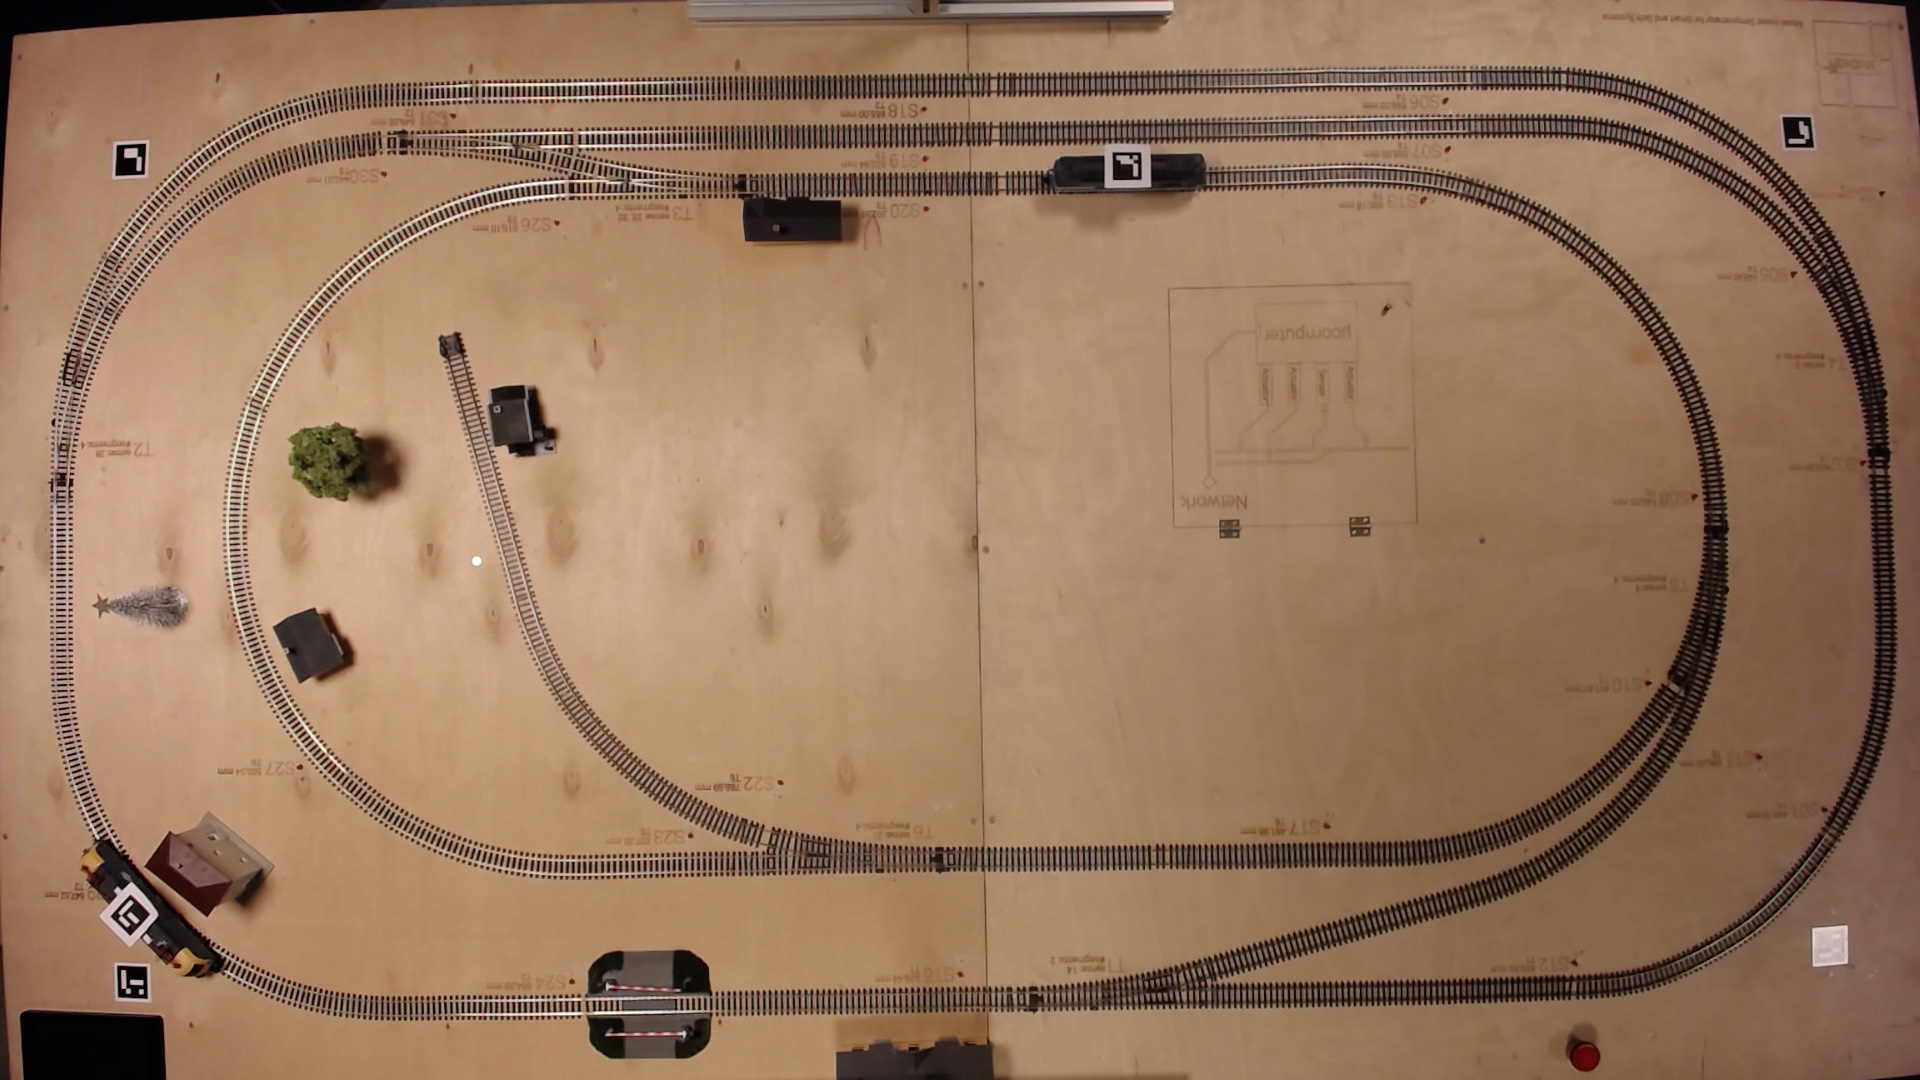
\includegraphics[width=150mm]{figures/modes3/overview.jpg}
	\caption{Railway system overview}
	\label{fig:overview}
\end{figure}

\section{Railway system basic components}
First of all I want to introduce the physical components and the basic process of the railway systems stub. There are 31 sections, with one blind track and 7 turnouts. The \ref{fig:layout} figure shows the layout of railway elements with corresponding segment ids. Over all a segment means either section or turnout.
\todo[inline]{Create more visible figure about layout}

\begin{figure}[h]
	\centering
	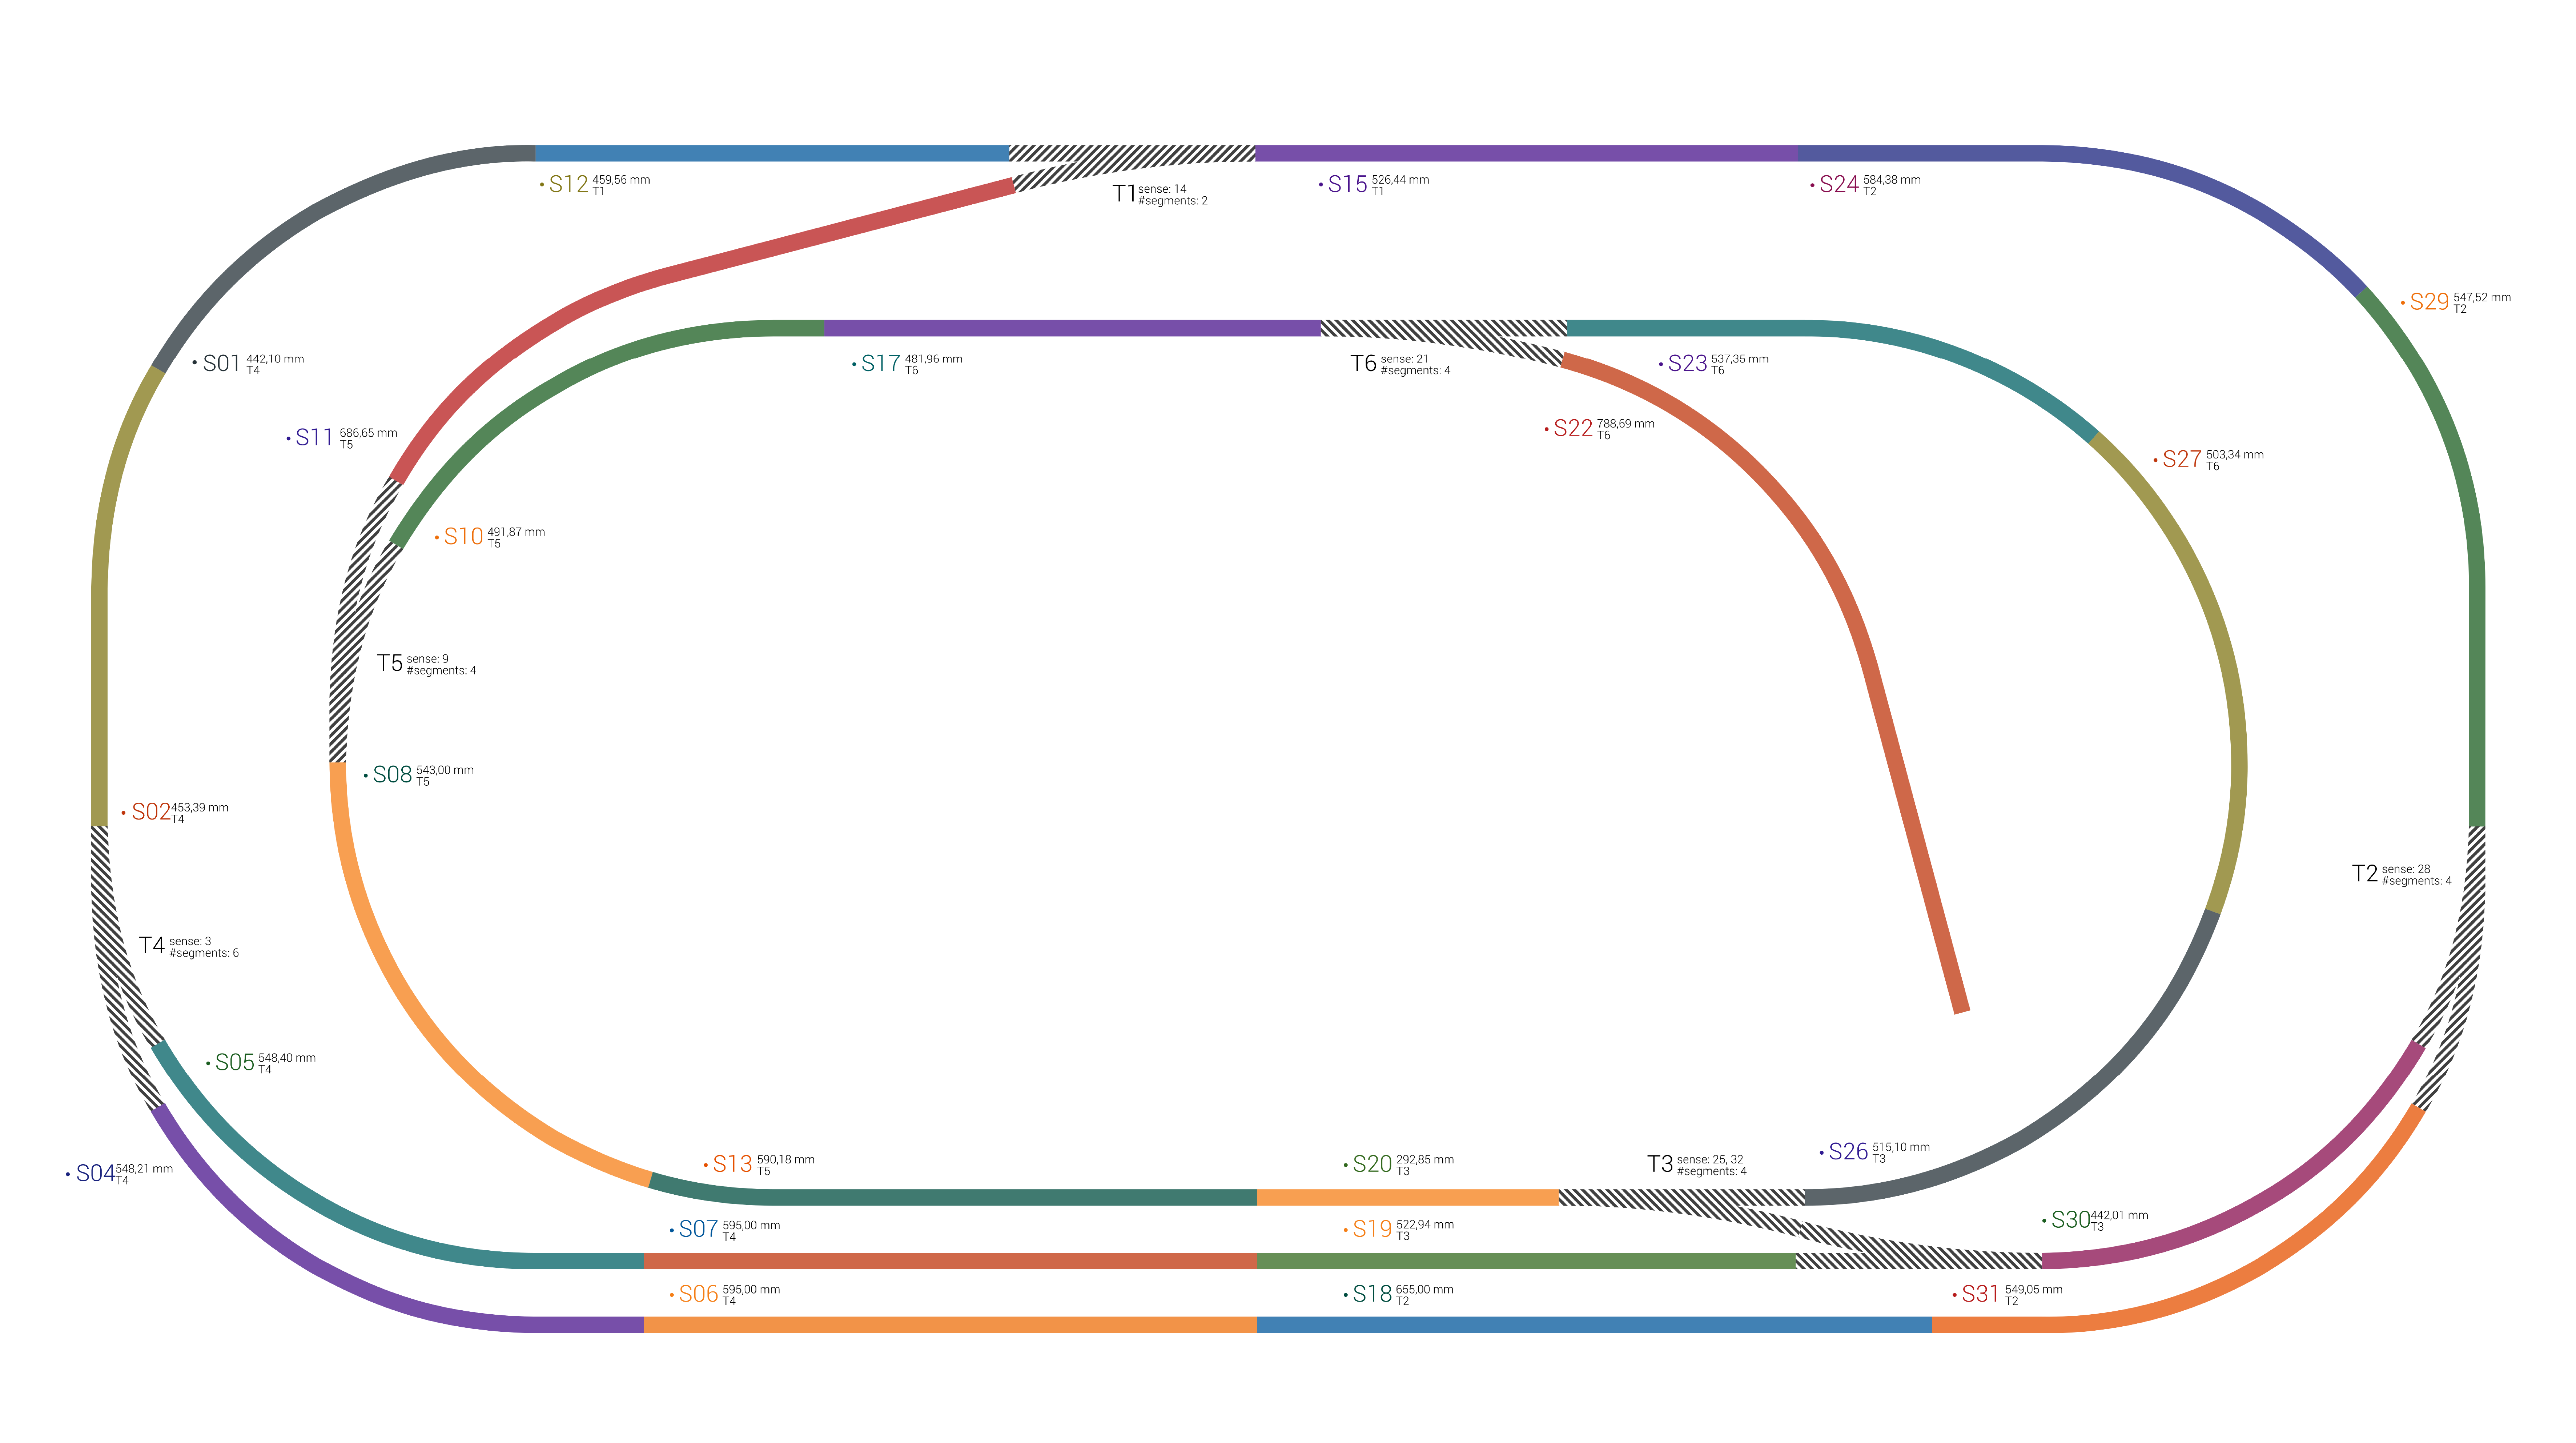
\includegraphics[width=150mm, keepaspectratio]{figures/modes3/layout2.png}
	\caption{Railway layout}
	\label{fig:layout}
\end{figure}

\paragraph{Section} 
First principal  element is a 15-20 cm long railroad. Each section is connected to 2 other sections, and wired to a command station which gives them sufficient power source for moving the trains. In the figure \ref{fig:layout} these sections are identified by \textit{SXX} strings, where \textit{XX} is two unique digits for this layout. Furthermore these numerals determines which bit shows this section's occupancy in the occupancy vector later (see section \ref{section:OccupancyDetection} for more information). On the \ref{fig:layout} figure for each section lengths and responsible BeagleBone Black ids are shown.

\paragraph{Turnout}
Second principal element is the turnout, which can differentiate 2 paths on the track as it can be seen on figure \ref{fig:turnoutDir}. The train which is going through a turnout can reach different sections depending on the state of the exact turnout. On the layout figure (\ref{fig:layout}) each of these elements are visible as gray dashed sections with the IDs. Each turnout ID starts with T and ends with a numeric (1..6). These IDs determines, which bit identifies the turnout's occupancy in the occupancy vector) and \textit{\#segments} as number of supervised sections by the BeagleBone Black (see section \ref{section:OccupancyDetection} for more information about occupancy vector).
\begin{figure}[!h]
	\centering
	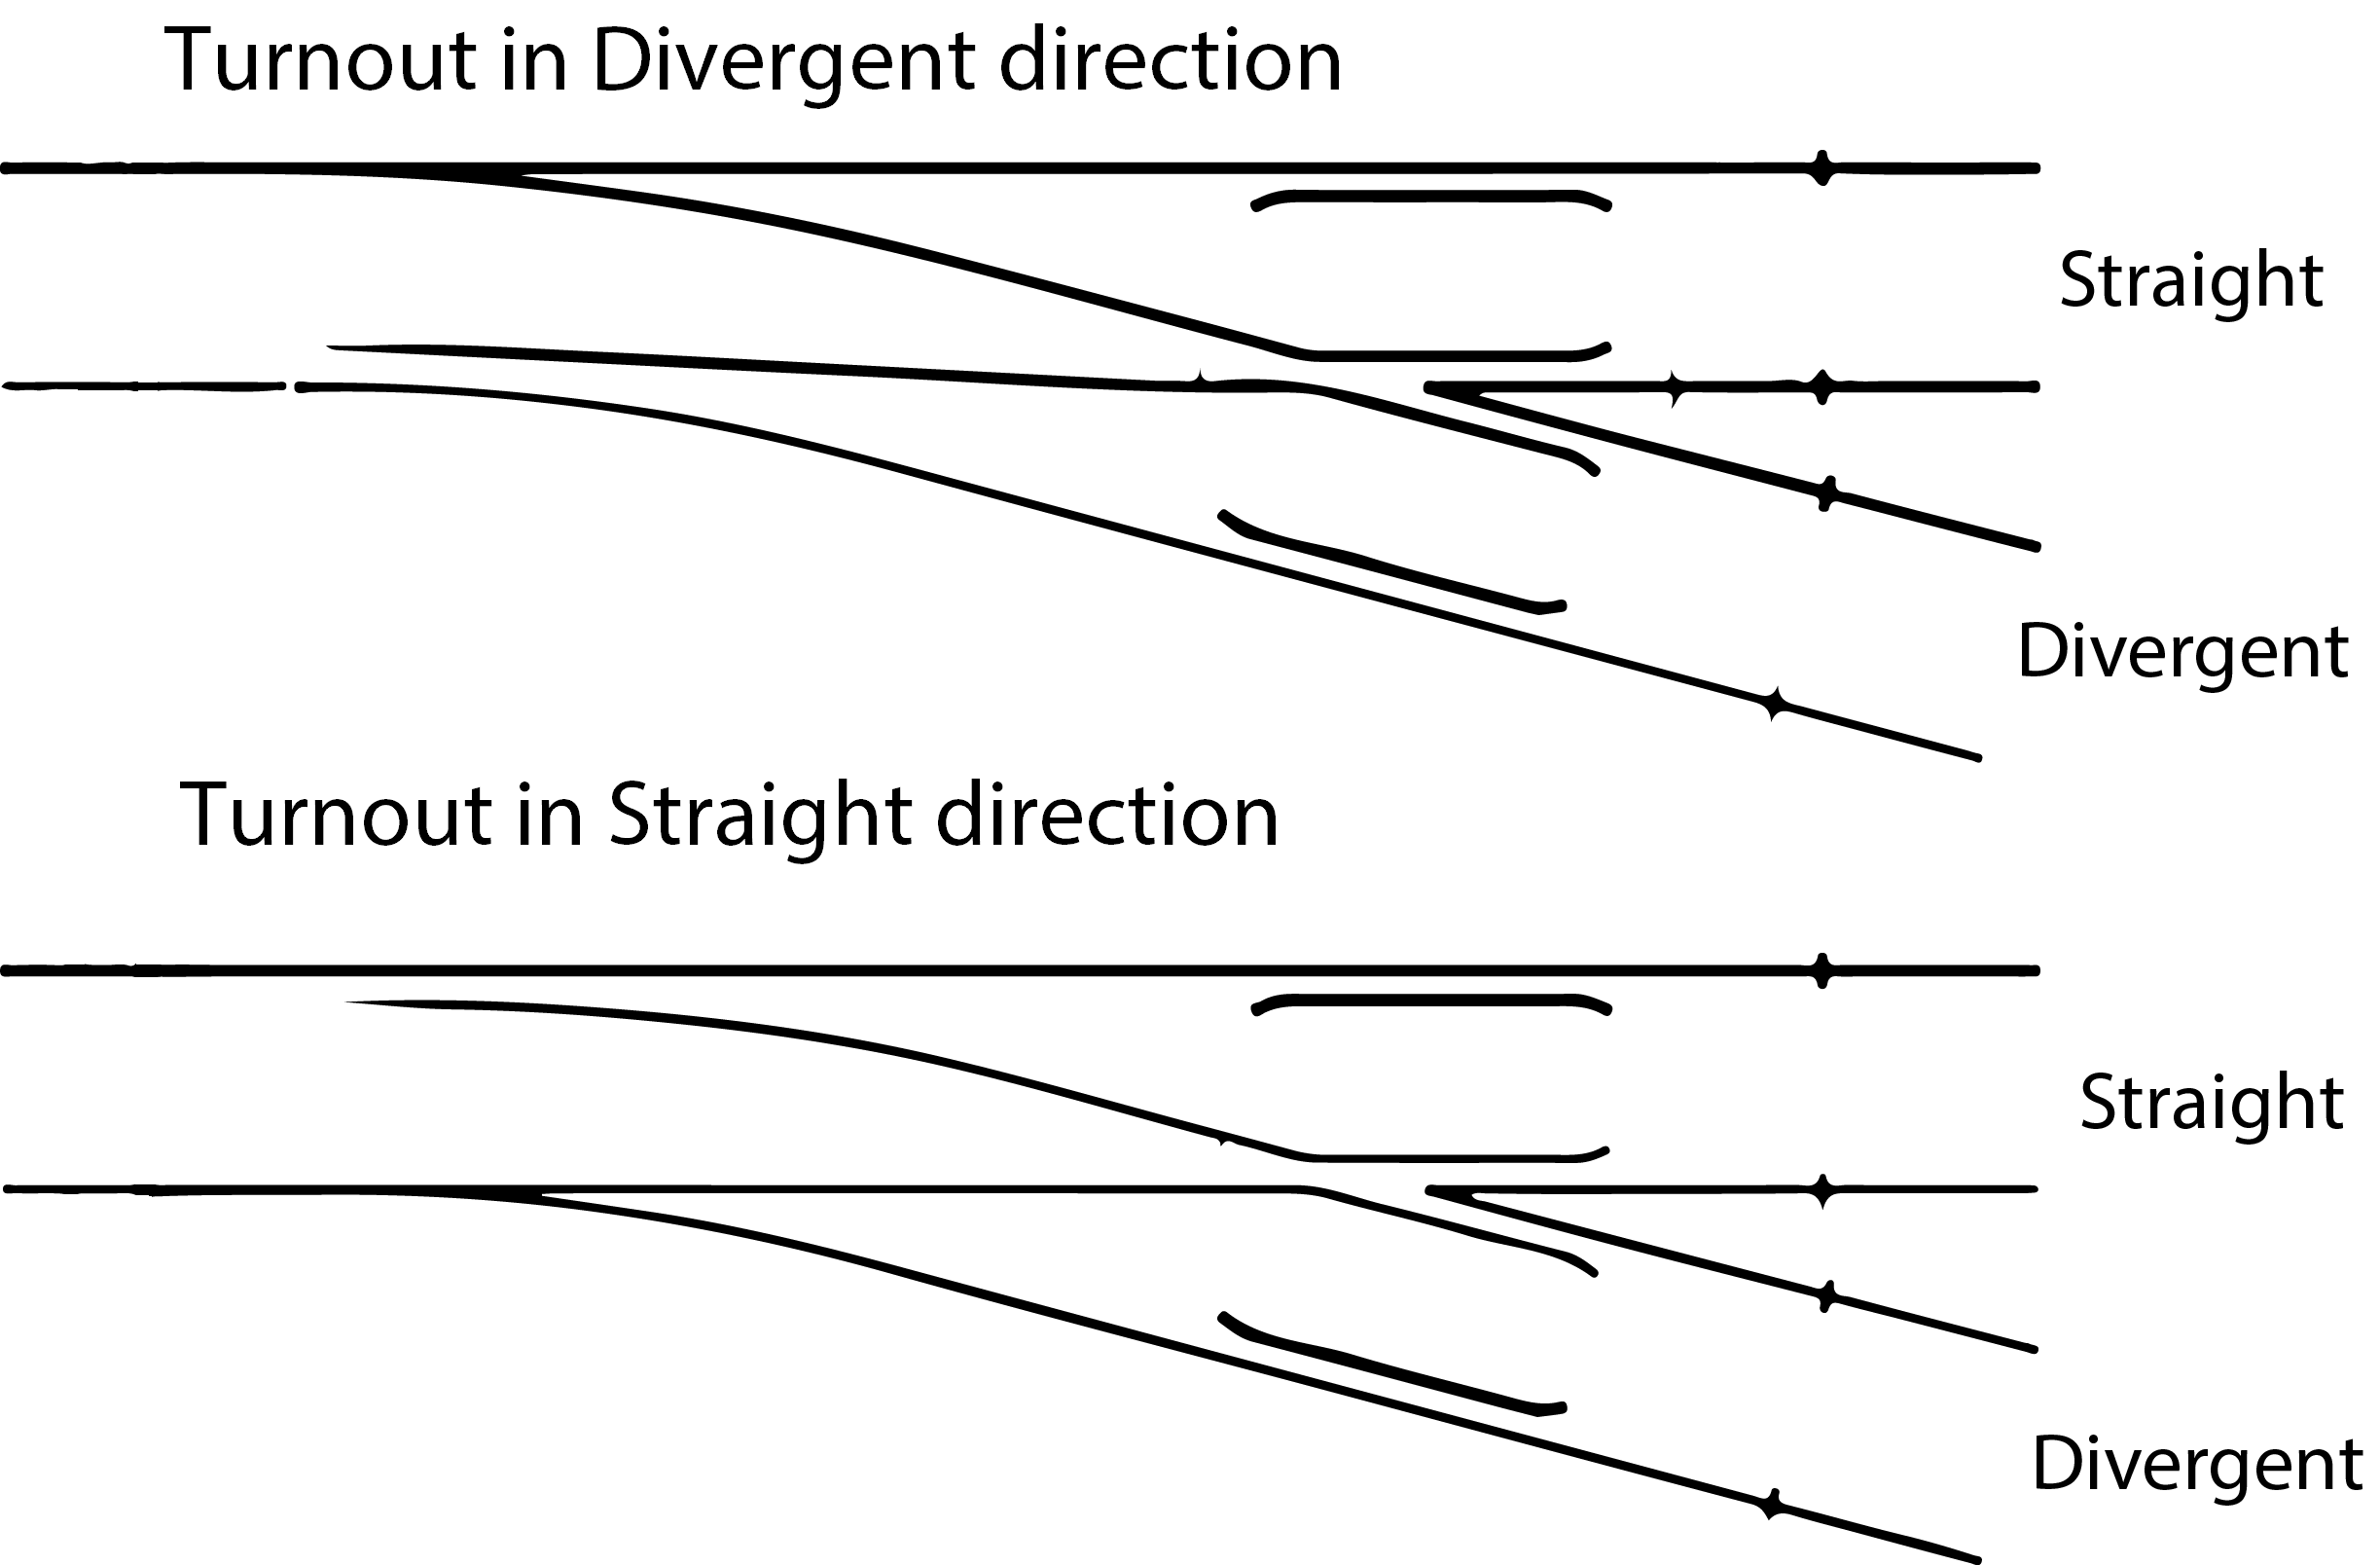
\includegraphics[width=150mm]{figures/modes3/turnout.png}
	\caption{Turnout directions}
	\label{fig:turnoutDir}
\end{figure}

\paragraph{Train} \label{par:trainScenarios}
There are 2 model trains in the system, which can move on the sections and turnouts. The first safety critical paradigm is to avoid a train collision on the track, for which the basic scenarios are the following. 

\todo[inline]{Move the collision scenarios to a new chapter}

First approach is that 2 trains are passing through the same turnout, from the same direction on different paths. It means that they are approaching the same section of the turnout, so they will collide like on the \ref{fig:LayoutT1-scenario1} figure.
\begin{figure}[!h]
	\centering
	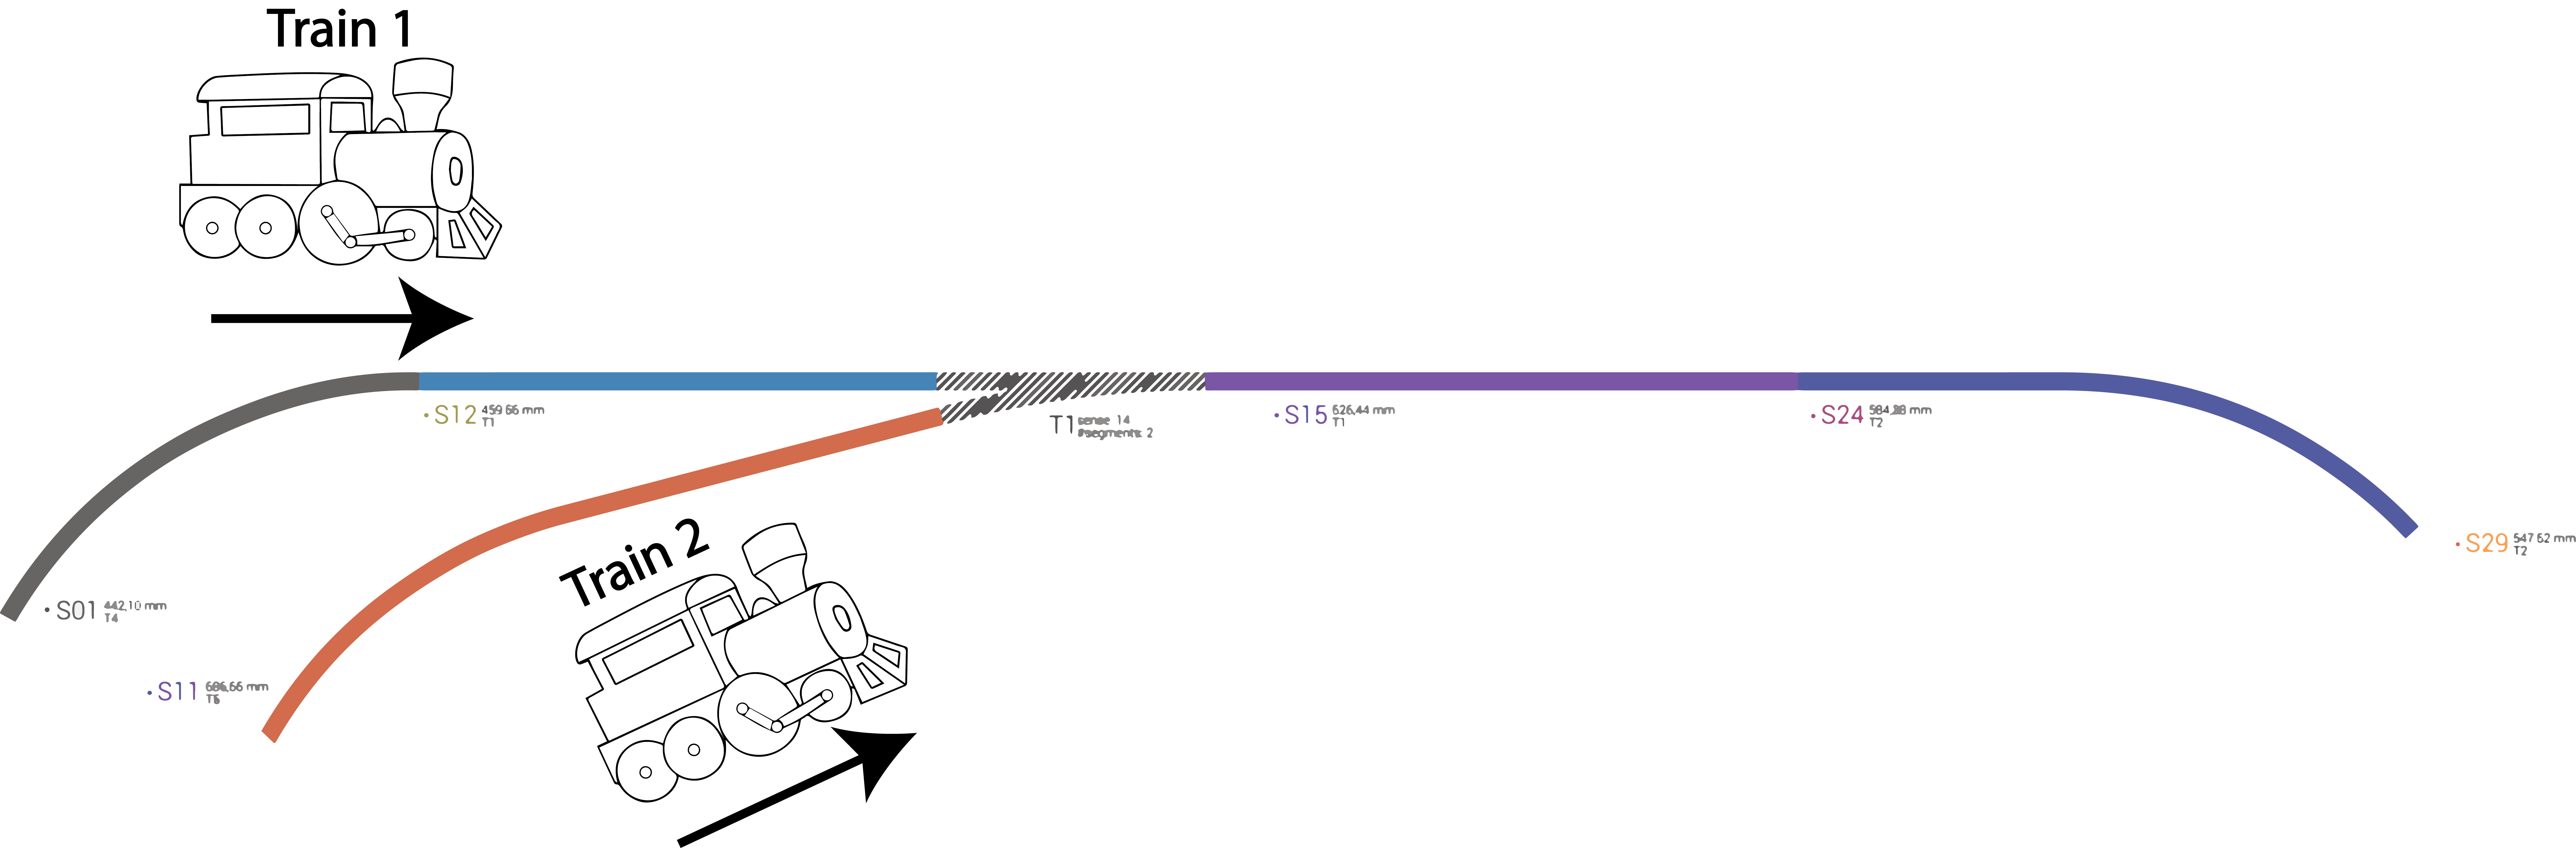
\includegraphics[width=150mm, keepaspectratio]{figures/modes3/layoutT1-scenario1.png}
	\caption{Turnout 1 collision scenario 1}
	\label{fig:LayoutT1-scenario1}
\end{figure}

Next possible scenario is shown in \ref{fig:LayoutT1-scenario2} figure, when \textit{Train 1} is going to the section where \textit{Train 2} is staying. Notice that no matter in which direction the \textit{Train 2} is moving or staying, it is a dangerous situation.
\begin{figure}[!h]
	\centering
	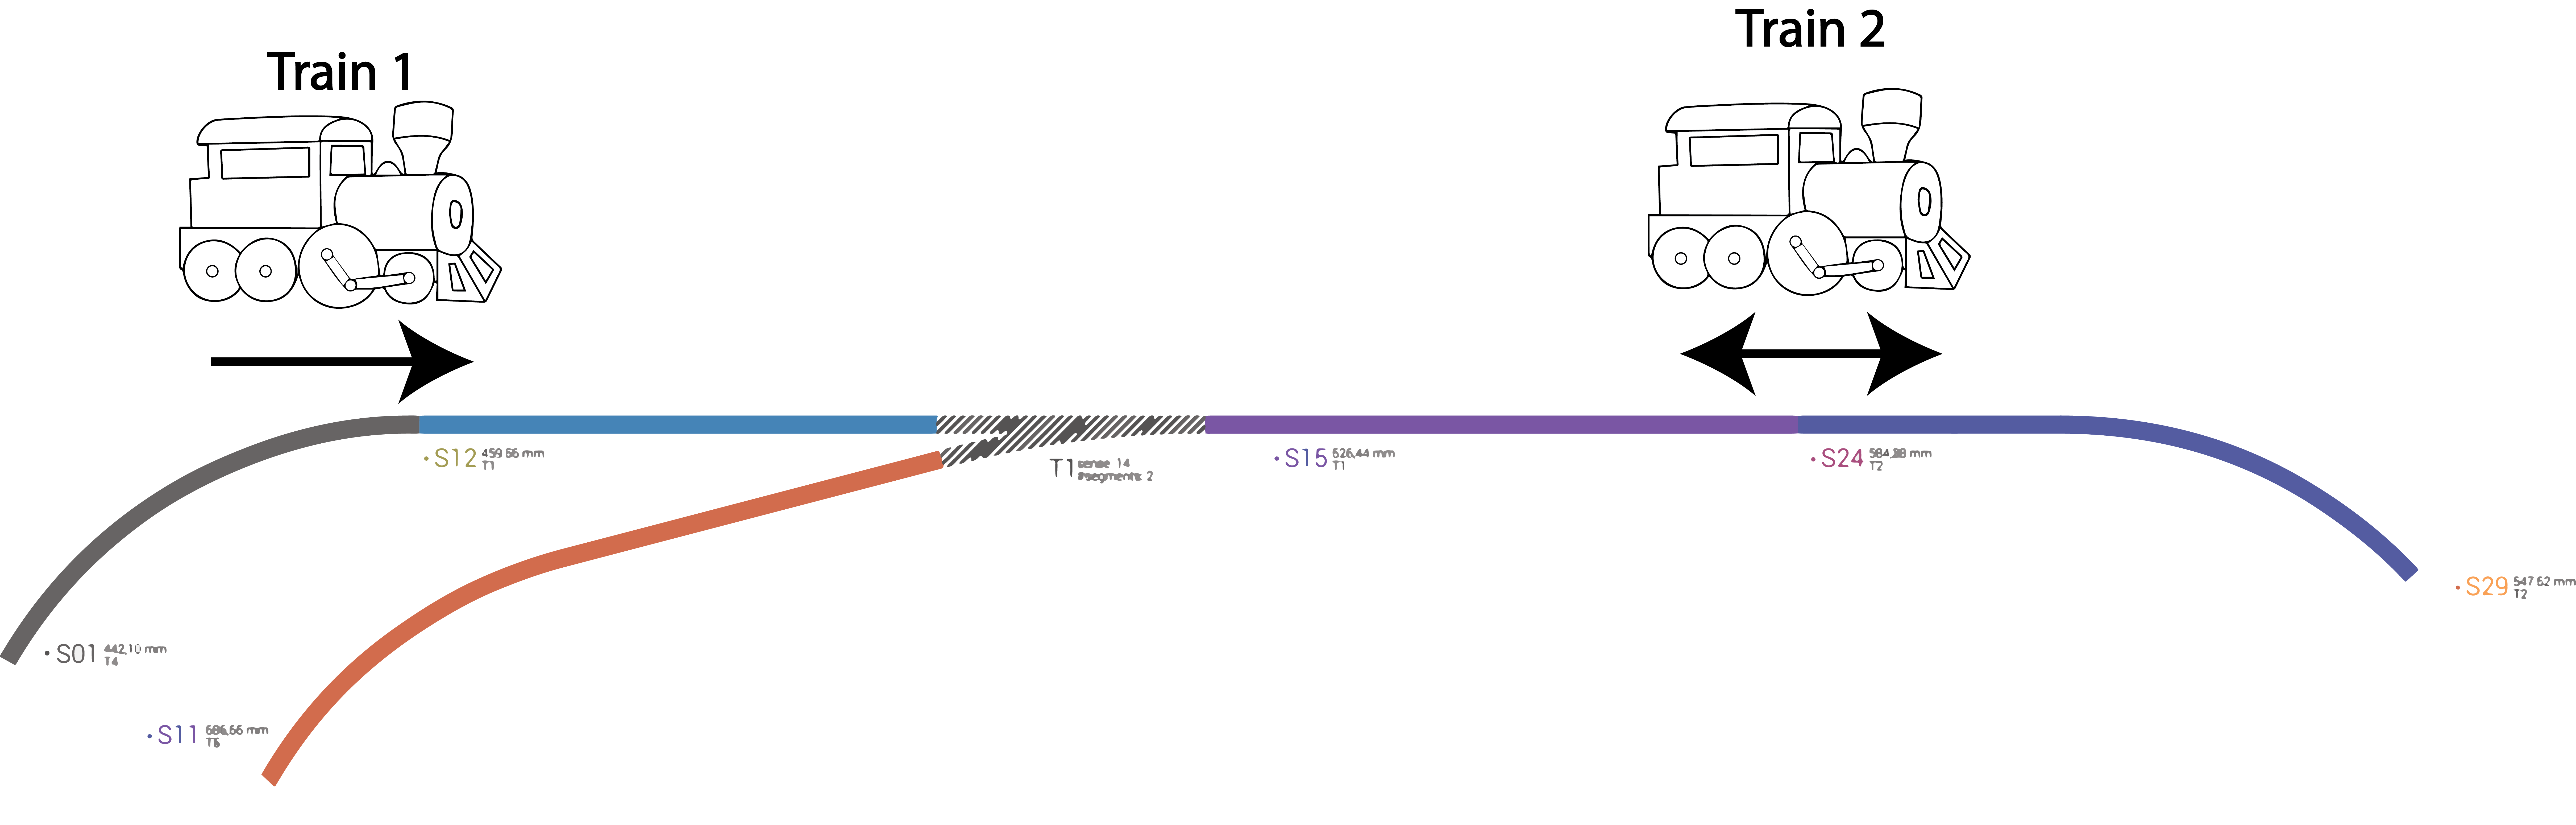
\includegraphics[width=150mm, keepaspectratio]{figures/modes3/layoutT1-scenario2.png}
	\caption{Turnout 1 collision scenario 2}
	\label{fig:LayoutT1-scenario2}
\end{figure}

\paragraph{Command Station}
Supply power source for the sections which provides tension for the trains on the track.

\paragraph{Controller}
In connection with the \textit{Command Station} an XPressNet protocol \footnote{More details about XPressNet Protocol \url{http://www.lenzusa.com/1newsite1/Manuals/xpressnet.pdf}} based controller is attached to the system. This component's purpose is setting the direction and speed for each train on the track.

\section{Hardware extensions}
The basic hardware environment is not sufficient for controlling and analyzing purposes, therefore additional hardware elements have been designed to satisfy these requirements. In this section these platforms will be described in details. (The \ref{appendix:HWPictures} appendix contains pictures about the elements.)
\todo[inline]{Check if these infos are necessary and where to put them}
For modeling purposes I have used MagicDraw with Sysml plugin \cite{SysML}.

\subsection{Data processing units}
\begin{figure}[h]
	\centering
	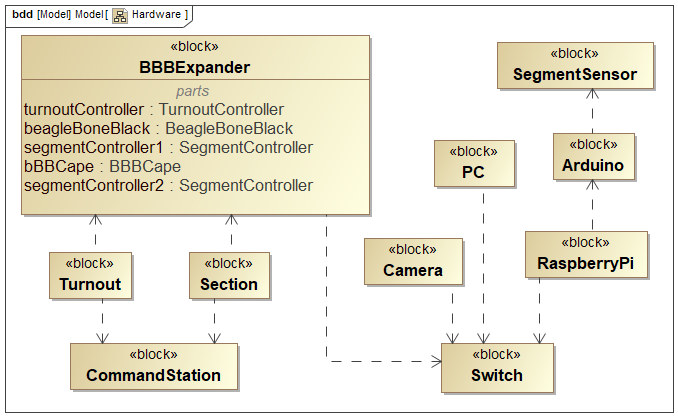
\includegraphics[width=150mm]{figures/modes3/Hardware.png}
	\caption{Hardware block definition diagram}
	\label{fig:Modes3HWBDD}
\end{figure}

\paragraph{BeagleBone Black (BBB)}
An industrial microcontroller platform which provides 4GB 8-bit eMMC on-board flash storage and 2x PRU 32-bit microcontrollers, which could satisfy the function for parallel monitoring. There are 6 BBB on the track connected to the railway, used for controlling and enabling/disabling each section.

\paragraph{Rapsberry Pi 3}
A Rapsberry Pi microcontroller is dedicated to handle most of the software components related to the Railway demonstrator system. It has twice as large computing capacity in RAM and also in CPU as BBB.

\paragraph{Arduino}
Dedicated hardware element for reading from the 6 DigiSens-8-S88 output data through S88 protocol (see \ref{par:SegmentSensor} section for details about this component). This communication layer requires proper timing conditions which the Arduino platform can satisfy.

\subsection{Custom hardware extensions}
\paragraph{BeagleBone Black cape and expanders}\label{par:BBBcape}
The BeagleBone Black components expect 5VDC power source instead of 12VDC which our power station supplies. Because of that reason a so called cape have been created for each controller. Additionally the need for easy-to-use ports to attach additional circuits to the main board also have come up. The expanders could be used to extend the functionality of one BeagleBone unit, which is on the figure \ref{fig:capeSysml}. 
\todo[inline]{More suitable figure here for BBB expendable interfaces}
\begin{figure}[!h]
	\centering
	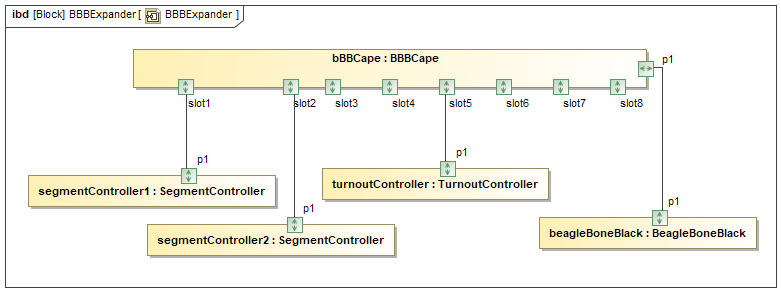
\includegraphics[width=150mm]{figures/modes3/BBBExpander.png}
	\caption{Layout and current attachment of cape and expander}
	\label{fig:capeSysml}
\end{figure}

Each cape have 8 general purpose expander slot, for which the pin layout is expressed in the following \ref{table:expander_pin_layout} table.

\begin{table}[!h]
	\caption{Pin layout}
	\label{table:expander_pin_layout}
	\begin{center}
		\renewcommand{\arraystretch}{1.5}
		\begin{tabu} to 0.5\textwidth { | X[c] | X[c] | X[c] | X[c] |}
			\hline
			pin3 & pin2 & pin1 & pin0 \\
			\hline
			3V3  & 5V  & Gnd  & 12V\\
			\hline
		\end{tabu}
	\end{center}
\end{table} 

\todo[inline]{Give proper details about G0-G15 pins, the table is not showing all of them like \url{https://github.com/FTSRG/BME-MODES3/wiki/HW-Expander-design}}  

The upper row of each connector is dedicated for GPIO connections. Two of the GPIO pins connected to the application processor and the remaining two GPIO pins are connected to the PRU unit.

With this setup, the PRU and the application processor can cooperate on hardware level.

\paragraph{Segment sensor}\label{par:SegmentSensor}
The DigiSens-8-S88 component is an off-the-shelf product, which can detect the occupancy for 8 segments. \footnote{More information about the product can be found here:\url{http://www.digitools.hu/termekek/erzekelok/digisens-8-s88}}.

\paragraph{Segment actuator}
Segment Actuator expanders are designed to stop a train on the corresponding segment. The concept behind this expander based on the Lenz Asymmetrical DCC and ABC functionality of train-decoders. \footnote{The following descriptions are based on \url{https://tonystrains.com/lenz-asymmetrical-dcc-and-abc/} article.}

%
%ABC (Automatic Brake Control) works in conjunction with Asymmetrical DCC. Asymmetrical DCC is a way to trigger ABC in the decoder. This gives the ability to stop trains at a section of the track with Asymmetrical DCC.

%\begin{figure}[!h]
%	\centering
%	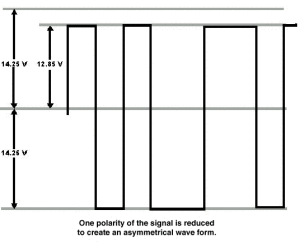
\includegraphics[width=100mm]{figures/modes3/DCC.png}
%	\caption{Asymmetric DCC voltages}
%	\label{fig:dcc}
%\end{figure}

%The Asymmetrical DCC signal is generated by offsetting one phase of the DCC signal. This signal then triggers the Automatic Brake Control in the decoder. This causes the engine to stop at the distance set up in the Constant Stopping Distance feature. We implemented this using five diodes. %connected in the form as shown in the figure below.
%\begin{figure}[h]
%	\centering
%	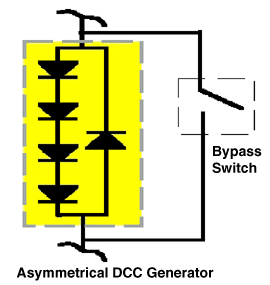
\includegraphics[width=50mm]{figures/modes3/abc.png}
%	\caption{Asymmetric DCC voltages}
%	\label{fig:abc}
%\end{figure}

The Segment Actuators uses this setup and also gives an interface (with GPIOs) to enable or disable this feature. Every Segment Actuator expander has two slots (A or B) and can enable or disable two segments. Each segment can be enabled setting two GPIOs to HIGH level, one connected to the PRU and one connected to the application processor.

\paragraph{Turnout actuator}
Turnout Actuator expanders can switch turnouts on the table between their states. Previously, we have managed to solve this with COTS (Commercial off-the-shelf) units, but in that case we were not able to query the position of the switch programmatically. This expander gives the ability for both switching the turnout and sensing its state.

The concept behind this unit is based on the fact, that turnout mechanism is working as a wire between the common (COM) pole and an other pole (STR or DIV) when switched in one position, therefore we can sense its state.

The electronic characteristics of the BeagleBone unit could not satisfy the switching process electrically, thus we had to use a micro-controller (an Atmega328 MCU). Also, the state-sensing process is based on Analog to Digital Converters, which are also integrated into the MCU.

\textbf{Usage}
The MCU has 2 inputs and 2 outputs connected to the expander connector as shown in the table below.
\begin{center}
	\renewcommand{\arraystretch}{1.5}
	\begin{tabu} to 1.0\textwidth {X[c] X[c] X[c] X[c]}
		\toprule
		Pin 0                                  & Pin 1                                   & Pin 2                           & Pin 3                             \\ \midrule
		Turnout switching to Straight position & Turnout switching to Divergent position & Turnout state sensing (Straing) & Turnout state sensing (Divergent) \\
		INPUT for the MCU                      & INPUT for hte MCU                       & OUTPUT for the MCU              & OUTPUT for the MCU                \\ \bottomrule
	\end{tabu}
\end{center}


\section{Software components}
\todo[inline]{update the figure with traindetector and delete physical controllers}
\begin{figure}[h]
	\centering
	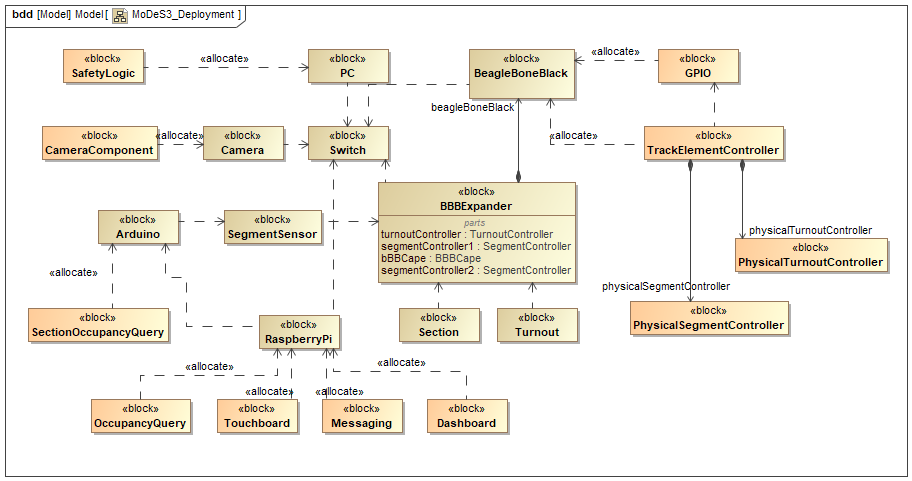
\includegraphics[width=150mm]{figures/modes3/MoDeS3_Deployment1.png}
	\caption{Software components deployment to hardware elements}
	\label{fig:Modes3Deployment}
\end{figure}

\subsection{Occupancy detection elements} \label{section:OccupancyDetection}
\paragraph{Section Occupancy Query}
Responsible for debouncing the 32bit long occupancy vector with proper timing conditions regarding S88 protocol and forward this 32bit to \textit{Occupancy Query} through usb connection. Computed data contains the occupancy information for each track element (section or turnout) per one bit.
\paragraph{Occupancy Query}
In connection with the \textit{Section Occupancy Query} process the occupancy state for the whole track. Only if the state has changed, it sends occupancy change message to the MQTT topic with the track element id and new occupancy state.

\subsection{Track segment control elements}
\paragraph{GPIO}
Handles the GPIO pin changes and commands for each extension point of the BBB cape (see \ref{par:BBBcape} section for details about BBB cape and expanders).
\paragraph{Track Element Controller}
On each BeagleBone Black microcontroller there is a controller, which executes the turnout and segment operations for the supervised sections. To satisfy this functionality this controller forwards commands to the corresponding Physical Segment or Turnout Controllers, which communicates with GPIO managers. Consequently with this platform specific software, we are able to enable or disable sections and set turnout directions.
\paragraph{Train Detector}
Train detector and locomotive length measurer using infrared sensors.

\subsection{Track control and supervisor elements}
\paragraph{XPressNet}
Protocol for sending messages to the \textit{Command Station} component, therefore we can extend the communication form for controlling the track. In the current layout there is a controller and web-based opportunity for controlling.
\paragraph{Dashboard}
Model railway track dashboard implementation, where we can manipulate the track elements. In Addition this component is instantiated only once, and up for the whole time while the track is in use. Consequently we can reach one common dashboard from the web and it contains the actual occupancy and track element status.
\paragraph{Touch board}
Dashboard for the model railway track, with focus on touchable elements, that can be controlled.
\paragraph{Safety Logic}
In the MODES$^3$ safety critical project we want to avoid the collision of model trains, therefore the safety logic software component detects these critical scenarios by Viatra Query \cite{Viatra} patterns and act the necessary action (for example disable a section).

\subsection{Messaging elements}
Each software component share information about the railroad system through the messaging software element, which is based on protobuf messages and provides high-level designed API with MQTT for this purpose. 
\begin{figure}[!h]
	\centering
	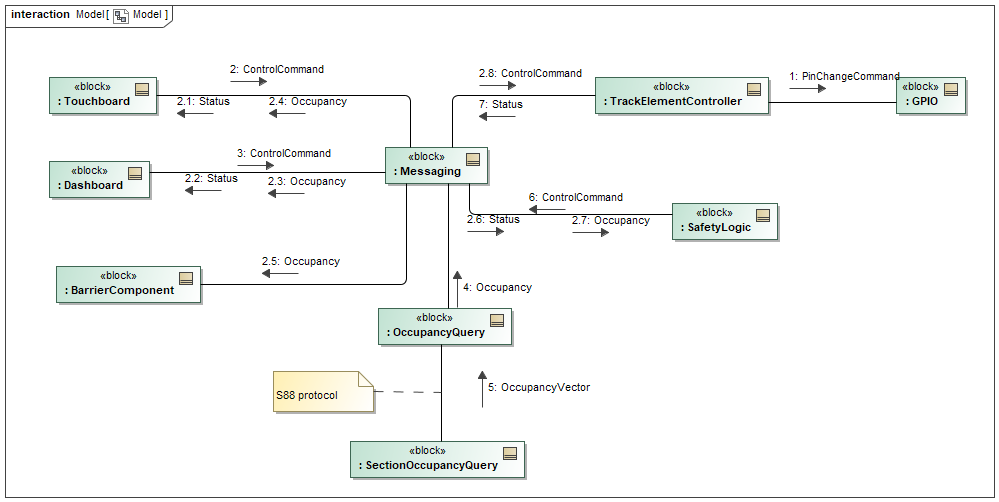
\includegraphics[width=150mm, keepaspectratio]{figures/modes3/CommunicationModel.png}
	\caption{Communication between software components}
	\label{fig:communicationModel}
\end{figure}

Separated topics are created for different information flow, and any component can subscribe for these topics. Basically on all topic, the information reporting is change based, so all components sending an information message to the dedicated topic when their state have changed (like occupancy changed or turnout changed). In opposite to that, there is a \textit{SendAllStatusCommand} which is a request for every component to send their actual status.

I will now list the specific MQTT topics and the connected software components to that, so basically what kind of information is flowing on them. (See software component connections on figure \ref{fig:communicationModel})

\paragraph{Segment Occupancy topic}
On this topic the \textit{Occupancy Query} component sending information whether an occupancy state is changed on any segment. (Notice that a segment can also be a section or a turnout too.) Most of the components are subscribed for this information topic so the \textit{Touch board}, \textit{DashBoard}, \textit{Barrier} (only for the supervised segments), \textit{Track Element Controller} and \textit{Safety Logic}.

\paragraph{Segment and Turnout Command topic}\label{par:MQTTTopicCommand}
Basically the \textit{Track Element Controller} process and accomplish these commands, and \textit{Touch board}, \textit{Dashboard} and \textit{Safety Logic} components can give these instructions.

\paragraph{Segment and Turnout Status topic}\label{par:MQTTTopicStatus}
For every command the \textit{Track Element Controller} will give a status acknowledgment message with the new state of the turnout or section. In this way the \textit{Touch board}, \textit{Dashboard} and \textit{Safety Logic} elements will be informed about the latest and current state.

\paragraph{CV topic}
The camera notification is communicated on that topic, which is received by the \textit{Safety Logic}.

\paragraph{ALL topic}
For this specific topic all the components in the system are subscribed, and information about train controlling and \textit{Command Station} related messages are shared.

\subsection{Complementary elements}
\paragraph{Barrier} 
Sends open/close commands to the barrier over the network, depending on the occupancy of supervised segments.
\paragraph{Leapmotion}
Software component for converting gestures into special movements for changing the speed of a specific train.

\section{Safety-critical functionalities}
\todo[inline]{Maybe figure of the Sw-Hw sysml for each paragraph}
\paragraph{Occupancy detection}\label{par:FunctionOccupancyDetection}
In order to know where are the trains on the track, we first must know which track elements (section or turnout) is occupied. This attribute can be determined whether the specific section has power consumption, which is used by train on it. The actual detection is made by the \textit{DigiSens-8-S88} sensing element. The demonstration railway system have four sensing element, and they are connected to an \textit{Arduino} S88 port. This microcontroller computes basic calculations by \textit{Section Occupancy Query} C++ software component and forwards the 32-bit occupancy vector information (actual state of every track element) to the \textit{Occupancy Query} via USB. The\textit{ Occupancy Query} Java component on the \textit{Rapsberry Pi} stores the previous occupancy state, and sends information to the \textit{Segment Occupancy} topic.

\paragraph{Track element controlling}\label{par:FunctionTEC}
For safety critical purposes in any collision scenario it is a good manner to disable all track elements, which is affected in the critical scenario. To make this switch possible, we have to cut the electric circle between the segment and \textit{Command Station}. The \textit{Section Controller} hardware element have been developed for changing a section,  the \textit{Turnout Controller} is responsible for changing a turnout. These hardware elements are attached to a \textit{BBB cape}, which is designed for supplying extension ports for BBB. In software point of view, through GPIO pins (specific file writing), we can give impulses from the BBB to the section or turnout. Therefore a \textit{GPIO manager} component is responsible for that in connection with the \textit{Track Element Controller component}. Both of them are Java components and deployed to the BBB microcontrollers.

\paragraph{Safety critical verification}
Because of the network communication, it is easy to connect a \textit{safety logic} in the system. In addition a camera component is reading the position of the trains on the track. If the \textit{Safety Logic} detects an unsafe scenario from the occupancy detection or camera, it switches off the affected elements by a \textit{Track Element Controller} signal.

\section{Requirements}
In this section I want to collect the specific requirements for the above described elements, not considering market products.

\paragraph{Custom hardware elements}
\begin{enumerate}[label=REQ-MODES-1-\arabic*, leftmargin=*, format=\small]
	\item The BeagleBone Black cape must supply 5VDC power source.
	\item The BeagleBone Black expander must provide further options to attach hardware elements. The purpose is to access application processor and PRU unit pins of BeagleBone Black.
	\item The Segment actuator must stop the train on given section immediately.
	\item The Turnout actuator shall switch the corresponding turnout between divergent and straight states.
	\item The Turnout actuator should sense the given turnout's actual state.
\end{enumerate}

\paragraph{Occupancy detection software elements}
\begin{enumerate}[label=REQ-MODES-2-\arabic*, leftmargin=*, format=\small]
	\item The Section Occupancy Query must collect the occupancy information together from all the segments on the track. 
	\item The Occupancy Query software element must determine the occupancy state change for each segment.
	\item The Occupancy Query software element must give a sign when an occupancy state changed for each segment.
\end{enumerate}

\paragraph{Track segment controller elements}
\begin{enumerate}[label=REQ-MODES-3-\arabic*, leftmargin=*, format=\small]
	\item The GPIO software element must change the GPIO pins between their states.
	\item The Track Element Controller must be able enable and disable sections with a specific command.
	\item The Track Element Controller must be able to change turnout directions in all states.
	\item The Train Detector must identify the length and the speed of a specific train.
\end{enumerate}

\paragraph{Track control and supervisor elements}
\begin{enumerate}[label=REQ-MODES-4-\arabic*, leftmargin=*, format=\small]
	\item The Dashboard must observe the track element states throughout the whole life-cycle.
	\item The Dashboard must be able to change all turnout states.
	\item The Dashboard must be able to enable and disable all segments on the track.
	\item The Safety Logic software must avoid safety critical scenarios on the track, like train collision. \todo[inline]{I should not use like here! Be more specific}
\end{enumerate}

%----------------------------------------------------------------------------
\chapter{Test design and documentation}
%----------------------------------------------------------------------------
\section{Test design techniques}

\todo[inline]{Extend this section with other used test design techniques}

The MoDeS$^3$ is a multi-layered, safety-critical application, which consist of off-the-self and custom made components also. As a complex system it is crucial to have a well-designed testing process and documentation which helps determine any problem in the system. For this purpose in the following chapter I will examine the possible and most suitable test approaches with a detailed test documentation.

\begin{figure}[!h]
	\centering
	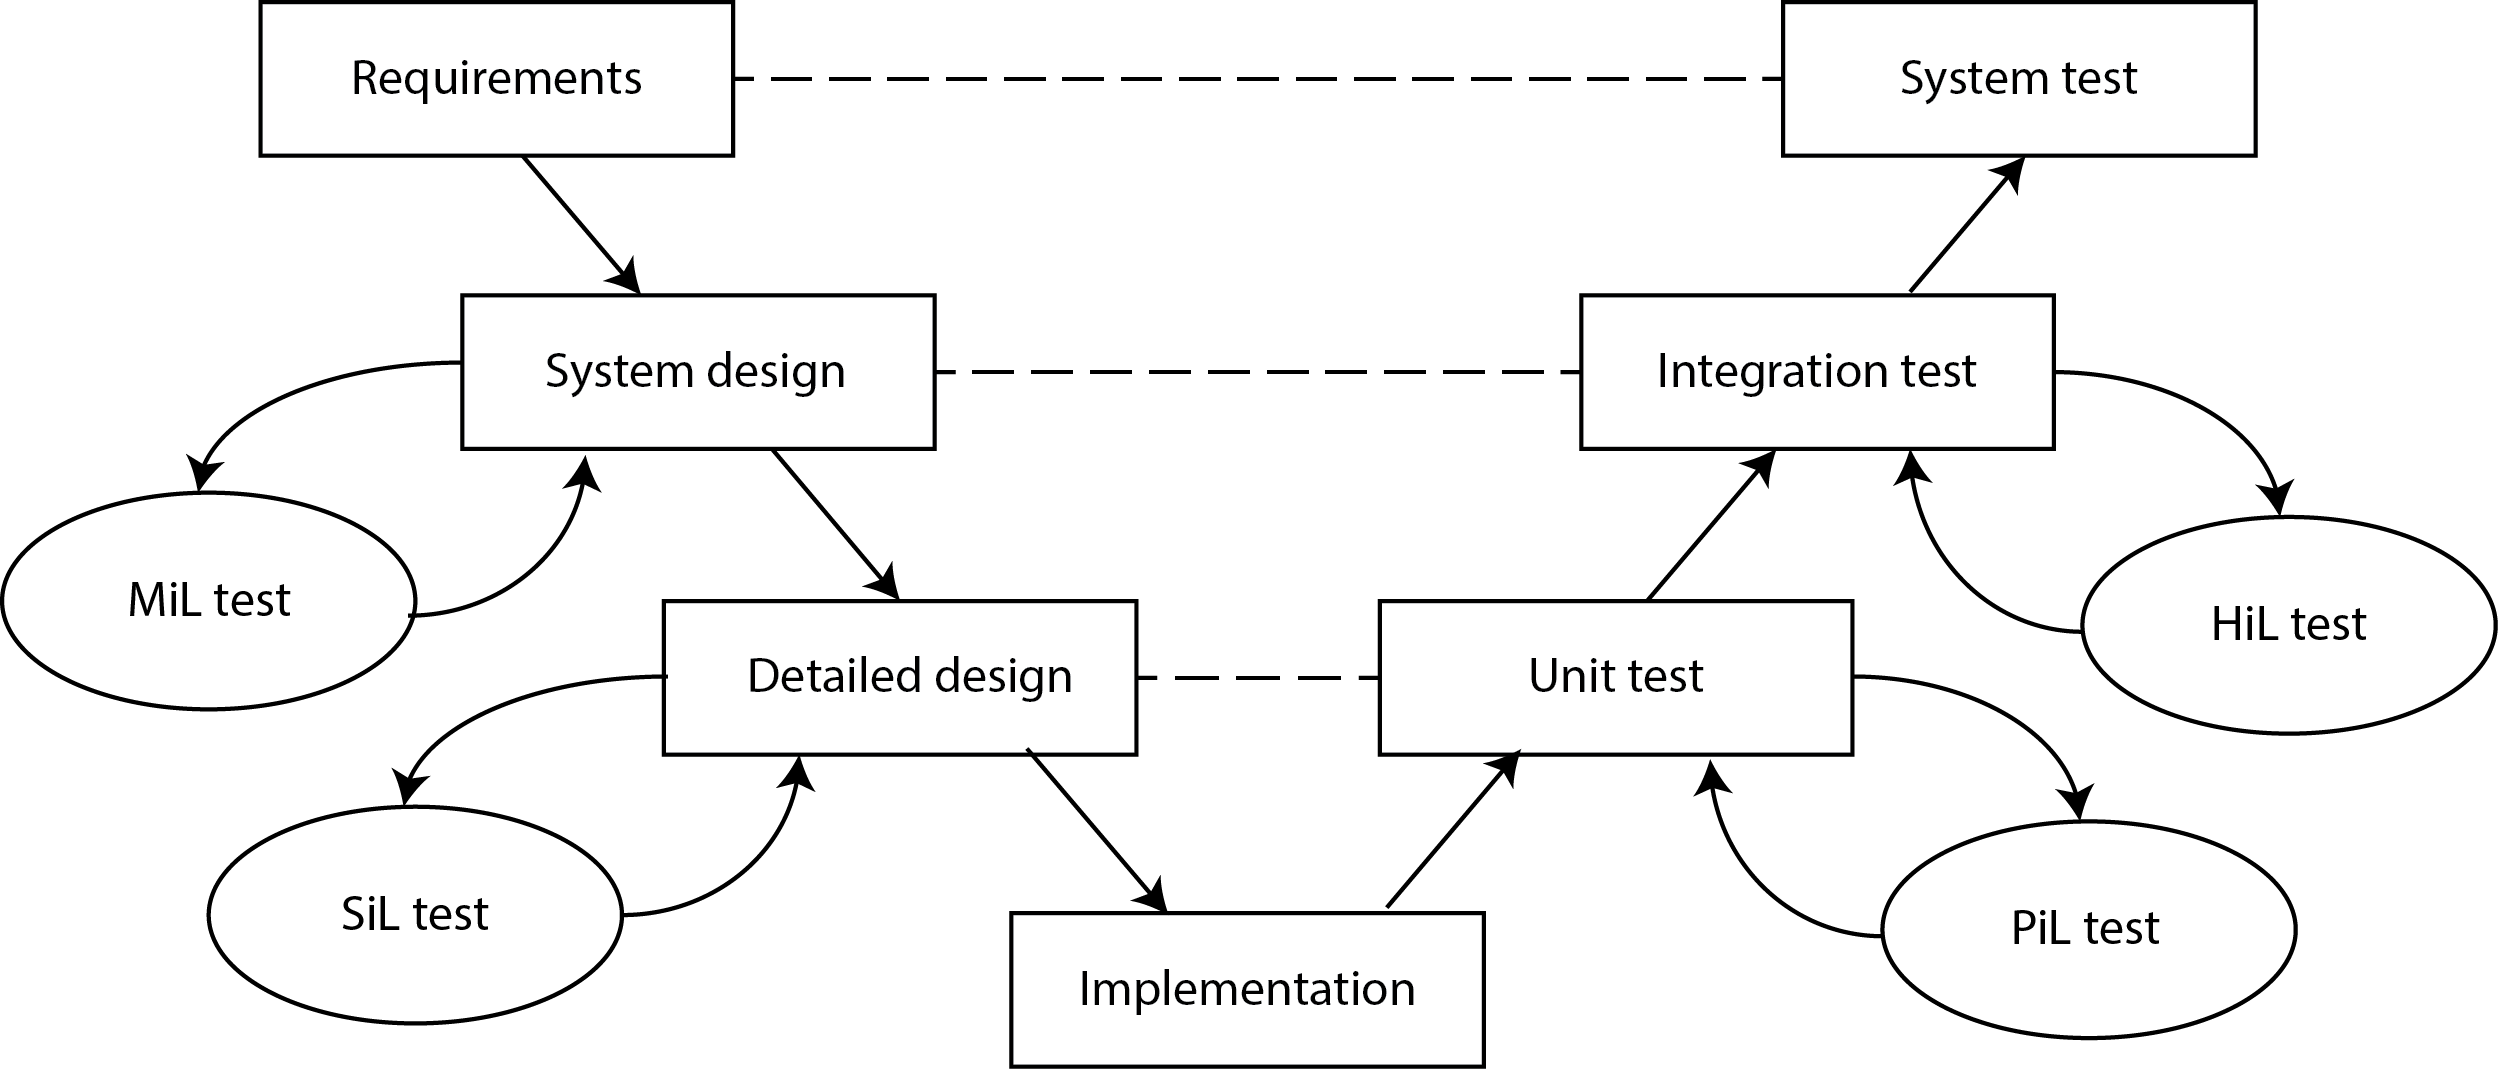
\includegraphics[width=150mm]{figures/testDesign/V_model.png}
	\caption{V-model}
	\label{fig:vModel}
\end{figure}

\subsection{V-model and testing levels}
Nowadays one of the most popular software development methodology is the V-model \cite{Vmodel} (shown on figure \ref{fig:vModel}), which defines four stages during the development and four verification steps accordingly (each step is shown with rectangles on the figure). In addition for making the development more effective for error-detection, there are four more steps defined for verifying our system's correctness, called test levels \cite{TestLevels} (shown with ellipses). While the development starts with an abstract \textbf{requirement analysis}, which declares the aim of our application, later on each step contains more detailed information. The second phase is about understanding the abstract user requirements and define the system's \textbf{functional specification} by the developers. During this phase our verification is based on \textbf{Model-in-the-Loop (MiL) testing}. The third phase contains all the low-level design and specific information about the application. From these design decisions, the \textbf{implementation} should be quite straight-forward or even it can be generated. During the \textbf{Software-in-the-Loop (SiL) testing}, the implementation will be verified for a subset of functionalities, which is depending on the system's purpose and requirements.
As of now our implementation is done and our design decisions are verified, we make sure with \textbf{unit tests} that our functions are serving their exact purposes. \textbf{Processor-in-the-Loop (PiL)} testing ensures that the computing processor at the bottom of the V-model works as expected. Then moving up in the V-model with \textbf{integration tests}, we are focusing on more abstract and complex components. In this phase we consider software and hardware elements also, completed with \textbf{Hardware-in-the-Loop (HiL)} testing. The last step is about verifying the complete system in real environment and check the high-level requirements.

\todo[inline]{give details about the used test design techniques}

\section{Test documentation}
During the test design phases of the MoDeS$^3$ I will follow a subset of the ISO 291119 standard \cite{IEEE13}.
First I will describe the documents in general, which will be later used in the MoDeS$^3$ test documentation process in section \autoref{TestDoc:MODES}. As of now the organizational and role details are irrelevant for this project, I will just give a short example for those. In the following sections, I will subtract the documentations into 3 phases, called Organizational, Test Management and Dynamic Test Documentation. 
\todo[inline]{redraw figure to something similar}
\begin{figure}[!h]
	\centering
	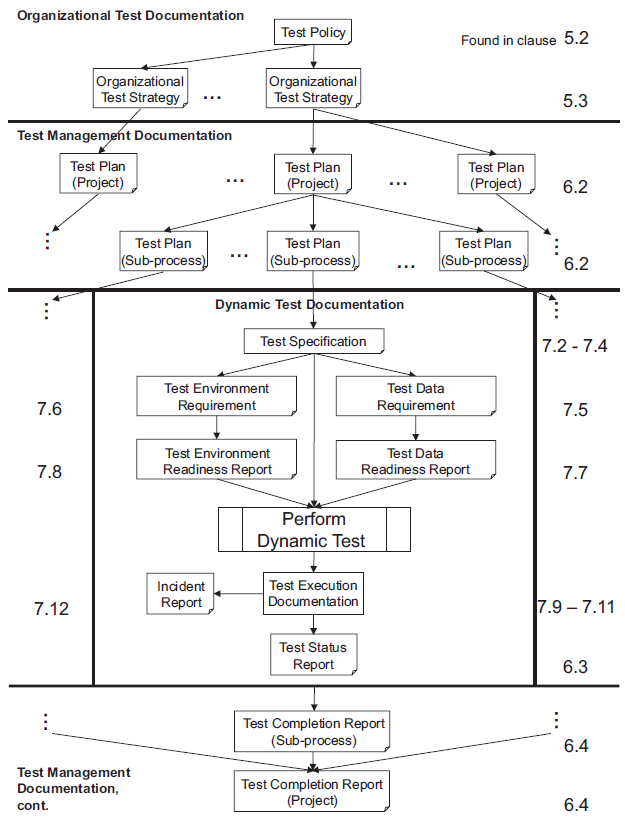
\includegraphics[width=150mm, keepaspectratio]{figures/testDesign/TestDoc.png}
	\caption{test Documentation Overview}
	\label{fig:TestDocOverview}
\end{figure}

\subsection{Organizational test documentation}
These general documents must be distributed organizational-wise and must be the same for every project within the organization. In according to this, during the test documentation the organization will be the MoDeS$^3$ team and the only project will be the above detailed railway system.

\paragraph{Test Policy}
Throughout the test development a Test Policy must contain the test principles and objectives for the whole organization. It clarifies what should be tested during development, but not how testing must be implemented. Furthermore it must define the provisions to be used for establishing, improving, maintaining and reviewing the test Policy.

\paragraph{Test Strategy}
A Test Strategy must define a proper guideline on how testing should be performed for all projects in the organization. In our case one Test Strategy is sufficient, but for an organization which have projects in different technical areas, can have a Test Strategy for each area. In latter case, the organization can define separate Test sub-processes to satisfy any special need for an area or project.

\todo[inline]{Do I need more details about test sub-processes?}

%\begin{enumerate}
%	\item Organizational Test Strategy
%	\begin{enumerate}
%		\item Introduction
%		\item General test strategy statements
%		\begin{enumerate}
%			\item Generic risk management
%			\item Test selection and prioritization
%			\item Test documentation and reporting
%			\item Test automation and tools
%			\item Configuration management of test work products
%			\item Incident management
%			\item Test sub-processes
%		\end{enumerate}
%	\end{enumerate}
%\end{enumerate}

\subsection{Test Management Documentation}
The Test Management Documentation is focusing on one project's planning and test evaluation. This group of documentation provides guidelines for Test Plan, Test Status Report and Test Completion Report.

\paragraph{Test Plan}
The collection of the test planning and test management documents is the Test Plan. It's scope be mapped to multiple projects, a single project or to sub-projects, where each Test Plan is dedicated for a sub-process (For example system test plan, integration software test plan, sub-system test plan, or unit software test plan). In a complex design structure it is advised to have a mapping tree document, which shows the relations between these Test Plans.

\paragraph{Test Status Report}
A report from the currently ongoing test process in a given reporting period is the Test Status Report. For example in an agile project it can be delivered at the end of the iteration. Although it is not necessarily a written document.

\paragraph{Test Completion Report}
As a summary of our test execution, a Test Completion Report can be provided for every test sub-process or for the whole project itself.

\subsection{Dynamic Test Documentation}
During the Dynamic Test Documentation phase the following documents are prepared:
\begin{itemize}
	\item Test Specification with sub-documents of:
	\begin{itemize}
		\item Test Design Specification
		\item Test Case Specification
		\item Test Procedure Specification
	\end{itemize}
	\item Test Data Requirements
	\item Test Environment Requirements
	\item Test Data Readiness Report
	\item Test Environment Readiness Report
	\item Test Execution Documentation with sub-documents of:
	\begin{itemize}
		\item Actual Result
		\item Test Results
		\item Test Execution Log
		\item Incident Report
	\end{itemize}
\end{itemize}
\todo[inline]{Figure of test docs hierarchy can be added here}

In the following sections, I will give a brief summary for each documentation.

\paragraph{Test Design Specification} \label{TestDoc:TDS}
The features and test conditions (derived from test basis) are collected in the Test Design Specification with the specific test cases and test procedures. These detailed test cases will be executed during testing process. 

Here we can create groups called \textit{feature sets} for those features which are connected together, then we can handle them independently.  A \textit{test condition} is aligned for each feature set and can be verified by a test case. Technically a test condition means a concrete state or representation of a feature. In addition on or more requirement can be referenced by a test case. In addition, to develop a more maintainable test document we must take care for the references from test cases to each requirement.

\paragraph{Test Case Specification}
One or more feature set with the defined test conditions and coverage items, constitutes a Test Case Specification.

\textit{Test coverage items} are obtained from a set of test conditions and specific test design technique. These items can be summarized in a list (describing test coverage items, test conditions and feature sets with proper priorities). From each test coverage item a \textit{Test case} can be derived, which verifies the correct implementation of a function. Regarding the possible number of test cases it can be collected into a list, table or database. Each test case should have a proper definition of dependencies. These are collected in \autoref{table:TestDoc:TestCases}.

\begin{table}[h]
	\caption{Details of a test case}
	\label{table:TestDoc:TestCases}
	\begin{center}
		\renewcommand{\arraystretch}{1.8}
		\begin{tabu} 
			to 0.9 \textwidth
			{  X[c]  X[c] }
			\toprule
			Aspect                     & Description                                                                                                                                               \\ \midrule
			Priority                   & Defines the execution order and importance between test cases. Higher priority test cases should be examined earlier then lower priorities                \\
			Traceability               & Reference the parent test coverage, condition item and the feature requirement                                                                            \\
			Preconditions              & Describes special states that must exists to execute the test case (Can be other test cases also)                                                         \\
			Inputs                     & A specific action which sets the test item into a state, where the actual and expected results can be compared                                            \\
			Expected result            & Specifies the expected output and behavior (with tolerances) of the test item which was in the precondition state and was modified with the proper inputs \\
			Actual result, test result & A description of test item outputs and a comparison between actual and expected results                                                                   \\ \bottomrule
		\end{tabu}
	\end{center}
\end{table} 

\paragraph{Test Procedure Specification}
Describes the precondition setup and test cases execution in the proper order with possible post evaluation activities.

Those test cases, which have the same purpose in the test item's property (for example precondition, test basis or even in the identified risk) can be collected into a \textit{Test set}. Typically this will reflect to one or more feature sets. For each \textit{Test set} the proper execution order is defined in the \textit{Test procedure} considering test case dependencies, preconditions, postconditions and other environment requirements.

\paragraph{Test Data Requirements}
Defines the required properties of the test data, which is used during test procedure execution. These requirements can be summarized with a list. In addition, this detailed test data requirements makes it more maintainable and traceable. 

\paragraph{Test Data Readiness Report} 
Gives a list of Test Data Requirements determining whether they are satisfied or not.

\paragraph{Test Environment Requirements}
Describes the required test environment properties, which are setting the test items into the expected test environment. These requirements can also be grouped by environment types like hardware, middleware, software, tools or security and may vary for each test case.

\paragraph{Test Environment Readiness Report}
Lists the fulfillment of Test Environment Requirements.

\paragraph{Actual Results}
After executing the selected test procedures, each test case's actual result (output state or behavior after the input actions) should be recorded. It may require full recording of the process with an automated tool also.

\paragraph{Test Result}
Determines if the actual results are corresponding to the expected results with the specified deviation or not. It is usually recorded as passed or failed, along with the actual results.

\paragraph{Test Execution Log}
Detailed documentation of one or more test procedure's execution. Can be represented in a list or table with measuring times and events of the test execution.

\paragraph{Test Incident Reporting}
If there is any deviation between the actual and expected results after each test procedure execution, we should create a dedicated Incident Report detailing the problems. These reports could contain a description of the problem with severity, date and possible risk information.

%%----------------------------------------------------------------------------
\chapter{Test evaluation}
%----------------------------------------------------------------------------

%----------------------------------------------------------------------------
\chapter{Summary}\label{chapter:Summary}
%----------------------------------------------------------------------------
During my thesis work, I got to know a test documentation standard \cite{IEEE13}. This approach was used to design a maintainable and detailed test plan for the MoDeS$^3$ project. The demonstrator system is a multi-layered application with off-the-shelf and custom hardware elements. Additionally for these microcontrollers, custom software components were developed to satisfy the required environment to control the track elements. Therefore I have detailed all the necessary software and hardware units to create a systematic test plan for the demonstrator system, which is mainly relies on the architecture and can be easily maintainable by the developers. The previously defined test cases was implemented in a safety-critical aspect also in unit, integration and system level.

I have found and detailed several improvable point in the \autoref{TestImpl:MODES}, which can take place in the future. These are especially component related implementation improvements, which can help testability in the following development phases.
%% !TeX spellcheck = hu_HU
% !TeX encoding = UTF-8
% !TeX program = xelatex
%----------------------------------------------------------------------------
\chapter{A \LaTeX-sablon használata}
%----------------------------------------------------------------------------

Ebben a fejezetben röviden, implicit módon bemutatjuk a sablon használatának módját, ami azt jelenti, hogy sablon használata ennek a dokumentumnak a forráskódját tanulmányozva válik teljesen világossá. Amennyiben a szoftver-keretrendszer telepítve van, a sablon alkalmazása és a dolgozat szerkesztése \LaTeX-ben a sablon segítségével tapasztalataink szerint jóval hatékonyabb, mint egy WYSWYG (\emph{What You See is What You Get}) típusú szövegszerkesztő esetén (pl. Microsoft Word, OpenOffice).

%----------------------------------------------------------------------------
\section{Címkék és hivatkozások}
%----------------------------------------------------------------------------
A \LaTeX~dokumentumban címkéket (\verb+\label+) rendelhetünk ábrákhoz, táblázatokhoz, fejezetekhez, listákhoz, képletekhez stb. Ezekre a dokumentum bármely részében hivatkozhatunk, a hivatkozások automatikusan feloldásra kerülnek.

A sablonban makrókat definiáltunk a hivatkozások megkönnyítéséhez. Ennek megfelelően minden ábra (\emph{figure}) címkéje \verb+fig:+ kulcsszóval kezdődik, míg minden táblázat (\emph{table}), képlet (\emph{equation}), fejezet (\emph{section}) és lista (\emph{listing}) rendre a \verb+tab:+, \verb+eq:+, \verb+sec:+ és \verb+lst:+ kulcsszóval kezdődik, és a kulcsszavak után tetszőlegesen választott címke használható. Ha ezt a konvenciót betartjuk, akkor az előbbi objektumok számára rendre a \verb+\figref+, \verb+\tabref+, \verb+\eqref+, \verb+\sectref+ és \verb+\listref+ makrókkal hivatkozhatunk. A makrók paramétere a címke, amelyre hivatkozunk (a kulcsszó nélkül). Az összes említett hivatkozástípus, beleértve az \verb+\url+ kulcsszóval bevezetett web-hivatkozásokat is a  \verb+hyperref+\footnote{Segítségével a dokumentumban megjelenő hivatkozások nem csak dinamikussá válnak, de színezhetők is, bővebbet erről a csomag dokumentációjában találunk. Ez egyúttal egy példa lábjegyzet írására.} csomagnak köszönhetően aktívak a legtöbb PDF-nézegetőben, rájuk kattintva a dokumentum megfelelő oldalára ugrik a PDF-néző vagy a megfelelő linket megnyitja az alapértelmezett böngészővel. A \verb+hyperref+ csomag a kimeneti PDF-dokumentumba könyvjelzőket is készít a tartalomjegyzékből. Ez egy szintén aktív tartalomjegyzék, amelynek elemeire kattintva a nézegető behozza a kiválasztott fejezetet.

%----------------------------------------------------------------------------
\section{Ábrák és táblázatok}
%----------------------------------------------------------------------------
Használjunk vektorgrafikus ábrákat, ha van rá módunk. PDFLaTeX használata esetén PDF formátumú ábrákat lehet beilleszteni könnyen, az EPS (PostScript) vektorgrafikus képformátum beillesztését a PDFLaTeX közvetlenül nem támogatja (de lehet konvertálni, lásd később). Ha vektorgrafikus formában nem áll rendelkezésünkre az ábra, akkor a  veszteségmentes PNG, valamint a veszteséges JPEG formátumban érdemes elmenteni.  Figyeljünk arra, hogy ilyenkor a képek felbontása elég nagy legyen ahhoz, hogy nyomtatásban is megfelelő minőséget nyújtson (legalább 300 dpi javasolt). A dokumentumban felhasznált képfájlokat a dokumentum forrása mellett érdemes tartani, archiválni, mivel ezek hiányában a dokumentum nem fordul újra. Ha lehet, a vektorgrafikus képeket vektorgrafikus formátumban is érdemes elmenteni az újrafelhasználhatóság (az átszerkeszthetőség) érdekében.

Kapcsolási rajzok legtöbbször kimásolhatók egy vektorgrafikus programba (pl. CorelDraw) és onnan nagyobb felbontással raszterizálva kimenthatők PNG formátumban. Ugyanakkor kiváló ábrák készíthetők Microsoft Visio vagy hasonló program használatával is: Visio-ból az ábrák közvetlenül PDF-be is menthetők.

Lehetőségeink Matlab ábrák esetén:
\begin{itemize}
	\item Képernyőlopás (\emph{screenshot}) is elfogadható minőségű lehet a dokumentumban, de általában jobb felbontást is el lehet érni más módszerrel.
	\item A Matlab ábrát a \verb+File/Save As+ opcióval lementhetjük PNG formátumban (ugyanaz itt is érvényes, mint korábban, ezért nem javasoljuk).
	\item A Matlab ábrát az \verb+Edit/Copy figure+ opcióval kimásolhatjuk egy vektorgrafikus programba is és onnan nagyobb felbontással raszterizálva kimenthatjük PNG formátumban (nem javasolt).
	\item Javasolt megoldás: az ábrát a \verb+File/Save As+ opcióval EPS \emph{vektorgrafikus} formátumban elmentjük, PDF-be konvertálva beillesztjük a dolgozatba.
\end{itemize}
Az EPS kép az \verb+epstopdf+ programmal\footnote{a korábban említett \LaTeX-disztribúciókban megtalálható} konvertálható PDF formátumba. Célszerű egy batch-fájlt készíteni az összes EPS ábra lefordítására az alábbi módon (ez Windows alatt működik).
\begin{lstlisting}
@echo off
for %%j in (*.eps) do (
echo converting file "%%j"
epstopdf "%%j"
)
echo done .
\end{lstlisting}

Egy ilyen parancsfájlt (\verb+convert.cmd+) elhelyeztük a sablon \verb+figures\eps+ könyvtárába, így a felhasználónak csak annyi a dolga, hogy a \verb+figures\eps+ könyvtárba kimenti az EPS formátumú vektorgrafikus képet, majd lefuttatja a \verb+convert.cmd+ parancsfájlt, ami PDF-be konvertálja az EPS fájlt.

Ezek után a PDF-ábrát ugyanúgy lehet a dokumentumba beilleszteni, mint a PNG-t vagy a JPEG-et. A megoldás előnye, hogy a lefordított dokumentumban is vektorgrafikusan tárolódik az ábra, így a mérete jóval kisebb, mintha raszterizáltuk volna beillesztés előtt. Ez a módszer minden -- az EPS formátumot ismerő -- vektorgrafikus program (pl. CorelDraw) esetén is használható.

A képek beillesztésére \az+\refstruc{sec:LatexTools}ben mutattunk be példát (\refstruc{fig:TeXstudio}). Az előző mondatban egyúttal az automatikusan feloldódó ábrahivatkozásra is láthatunk példát. Több képfájlt is beilleszthetünk egyetlen ábrába. Az egyes képek közötti horizontális és vertikális margót metrikusan szabályozhatjuk (\refstruc{fig:HVSpaces}). Az ábrák elhelyezését számtalan tipográfiai szabály egyidejű teljesítésével a fordító maga végzi, a dokumentum írója csak preferenciáit jelezheti a fordító felé (olykor ez bosszúságot is okozhat, ilyenkor pl. a kép méretével lehet játszani).

\begin{figure}[!ht]
	\centering
	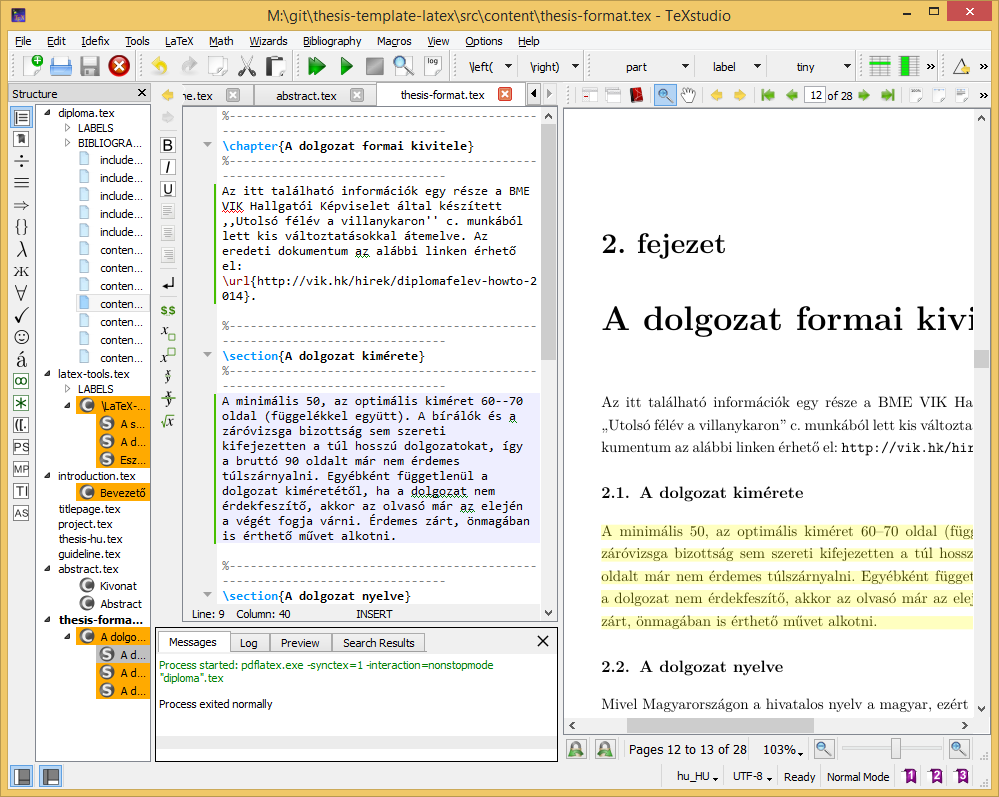
\includegraphics[width=67mm, keepaspectratio]{figures/TeXstudio.png}\hspace{1cm}
	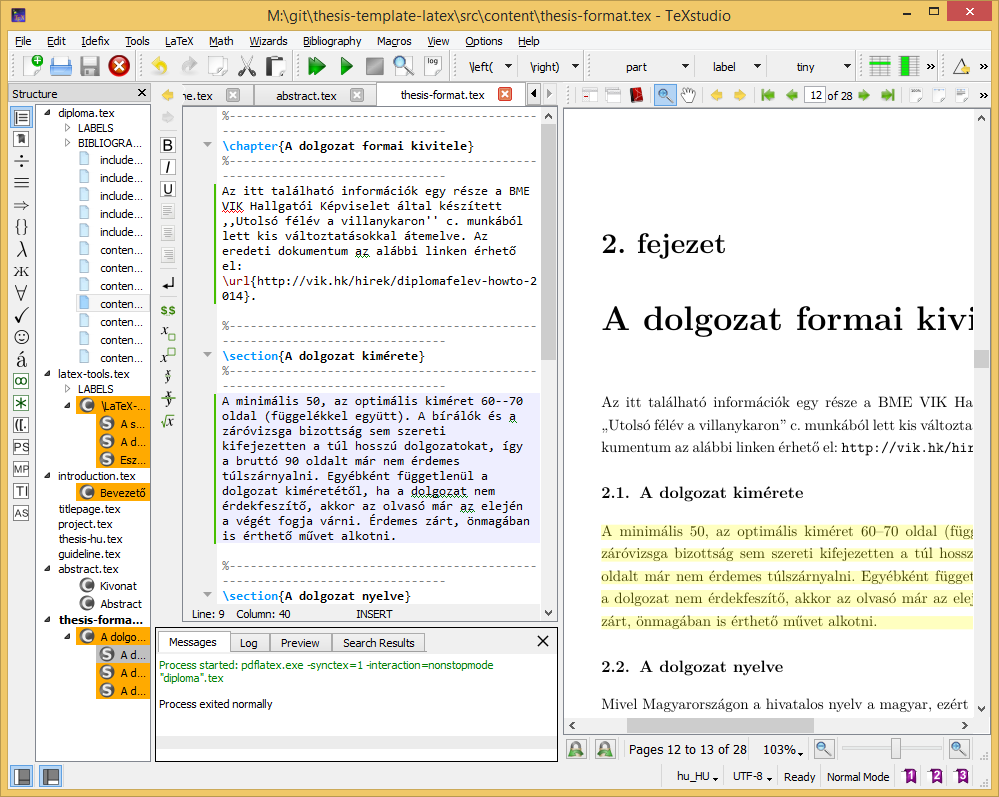
\includegraphics[width=67mm, keepaspectratio]{figures/TeXstudio.png}\\\vspace{5mm}
	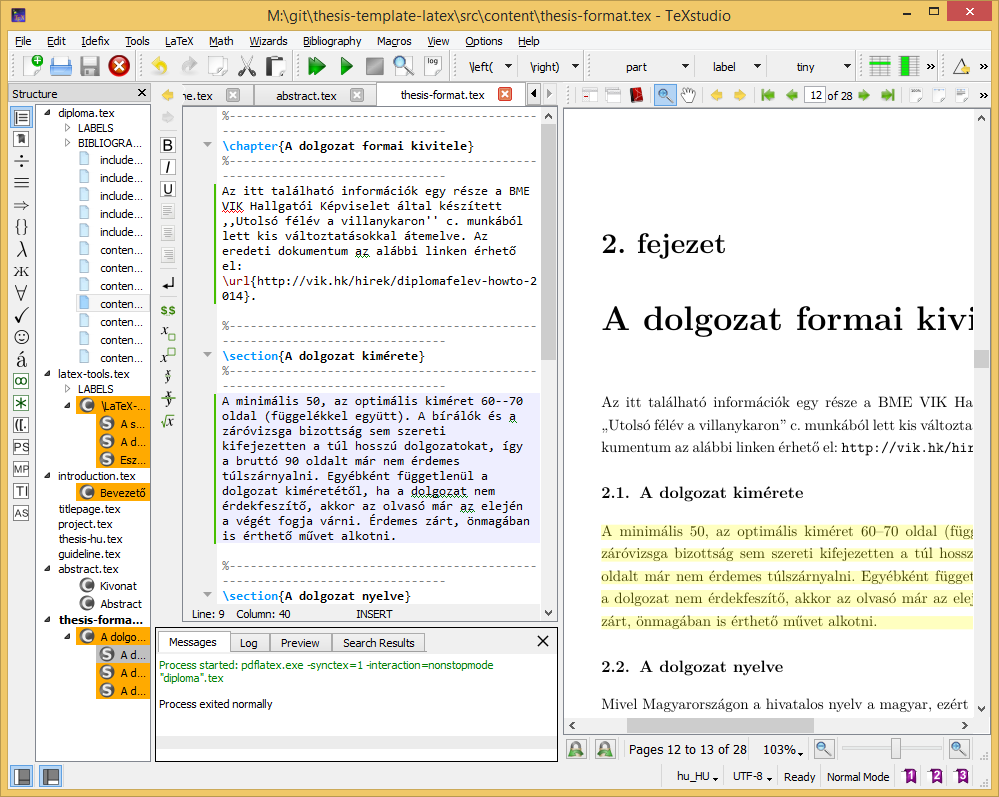
\includegraphics[width=67mm, keepaspectratio]{figures/TeXstudio.png}\hspace{1cm}
	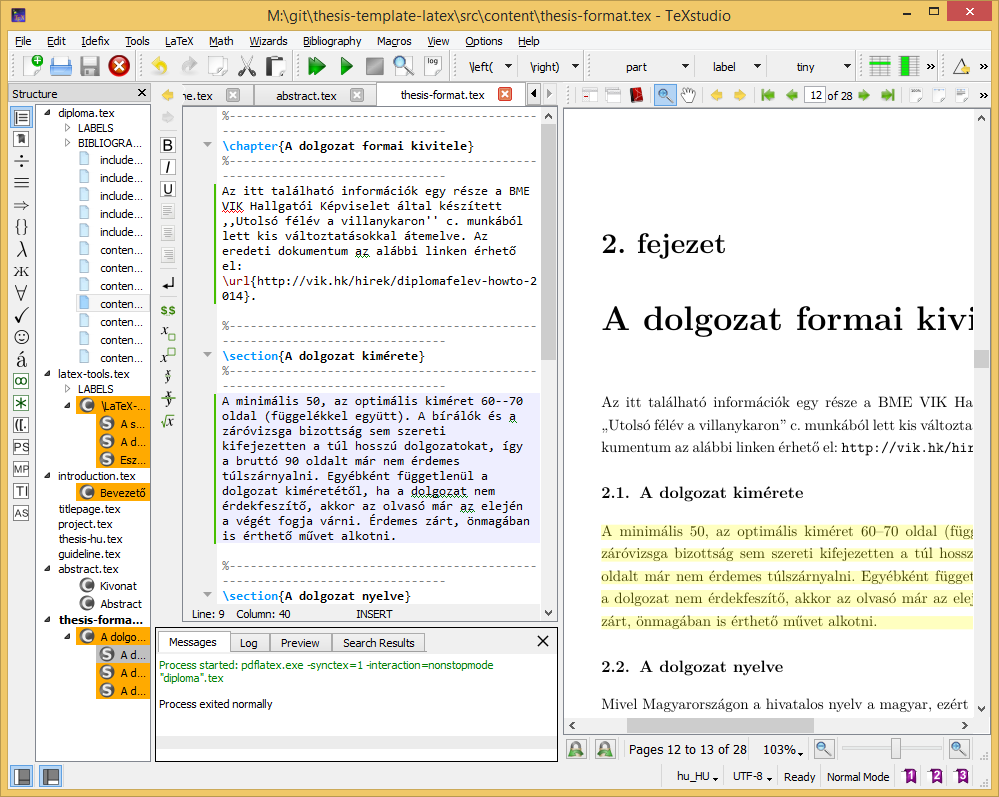
\includegraphics[width=67mm, keepaspectratio]{figures/TeXstudio.png}
	\caption{Több képfájl beillesztése esetén térközöket is érdemes használni.}
	\label{fig:HVSpaces}
\end{figure}

A táblázatok használatára \aref{tab:TabularExample}~táblázat mutat példát. A táblázatok formázásához hasznos tanácsokat találunk a \verb+booktabs+ csomag dokumentációjában.

\begin{table}[ht]
	\footnotesize
	\centering
	\begin{tabular}{ l c c }
		\toprule
		Órajel & Frekvencia & Cél pin \\
		\midrule
		CLKA & 100 MHz & FPGA CLK0\\
		CLKB & 48 MHz  & FPGA CLK1\\
		CLKC & 20 MHz  & Processzor\\
		CLKD & 25 MHz  & Ethernet chip \\
		CLKE & 72 MHz  & FPGA CLK2\\
		XBUF & 20 MHz  & FPGA CLK3\\
		\bottomrule
	\end{tabular}
	\caption{Az órajel-generátor chip órajel-kimenetei.}
	\label{tab:TabularExample}
\end{table}


%----------------------------------------------------------------------------
\section{Felsorolások és listák}
%----------------------------------------------------------------------------
Számozatlan felsorolásra mutat példát a jelenlegi bekezdés:
\begin{itemize}
	\item \emph{első bajusz:} ide lehetne írni az első elem kifejését,
	\item \emph{második bajusz:} ide lehetne írni a második elem kifejését,
	\item \emph{ez meg egy szakáll:} ide lehetne írni a harmadik elem kifejését.
\end{itemize}

Számozott felsorolást is készíthetünk az alábbi módon:
\begin{enumerate}
	\item \emph{első bajusz:} ide lehetne írni az első elem kifejését, és ez a kifejtés így néz ki, ha több sorosra sikeredik,
	\item \emph{második bajusz:} ide lehetne írni a második elem kifejését,
	\item \emph{ez meg egy szakáll:} ide lehetne írni a harmadik elem kifejését.
\end{enumerate}
A felsorolásokban sorok végén vessző, az utolsó sor végén pedig pont a szokásos írásjel. Ez alól kivételt képezhet, ha az egyes elemek több teljes mondatot tartalmaznak.

Listákban a dolgozat szövegétől elkülönítendő kódrészleteket, programsorokat, pszeudo-kódokat jeleníthetünk meg (\ref{lst:Example}.~kódrészlet).
\begin{lstlisting}[caption=A fenti számozott felsorolás \LaTeX-forráskódja,label=lst:Example]
\begin{enumerate}
	\item \emph{els(*@ő@*) bajusz:} ide lehetne írni az els(*@ő@*) elem kifejését,
	és ez a kifejtés így néz ki, ha több sorosra sikeredik,
	\item \emph{második bajusz:} ide lehetne írni a második elem kifejését,
	\item \emph{ez meg egy szakáll:} ide lehetne írni a harmadik elem kifejését.
\end{enumerate}
\end{lstlisting}
A lista keretét, háttérszínét, egész stílusát megválaszthatjuk. Ráadásul különféle programnyelveket és a nyelveken belül kulcsszavakat is definiálhatunk, ha szükséges. Erről bővebbet a \verb+listings+ csomag hivatalos leírásában találhatunk.

%----------------------------------------------------------------------------
\section{Képletek}
%----------------------------------------------------------------------------
Ha egy formula nem túlságosan hosszú, és nem akarjuk hivatkozni a szövegből, mint például a $e^{i\pi}+1=0$ képlet, \emph{szövegközi képletként} szokás leírni. Csak, hogy másik példát is lássunk, az $U_i=-d\Phi/dt$ Faraday-törvény a $\rot E=-\frac{dB}{dt}$ differenciális alakban adott Maxwell-egyenlet felületre vett integráljából vezethető le. Látható, hogy a \LaTeX-fordító a sorközöket betartja, így a szöveg szedése esztétikus marad szövegközi képletek használata esetén is.

Képletek esetén az általános konvenció, hogy a kisbetűk skalárt, a kis félkövér betűk ($\mathbf{v}$) oszlopvektort -- és ennek megfelelően $\mathbf{v}^T$ sorvektort -- a kapitális félkövér betűk ($\mathbf{V}$) mátrixot jelölnek. Ha ettől el szeretnénk térni, akkor az alkalmazni kívánt jelölésmódot célszerű külön alfejezetben definiálni. Ennek megfelelően, amennyiben $\mathbf{y}$ jelöli a mérések vektorát, $\mathbf{\vartheta}$ a paraméterek vektorát és $\hat{\mathbf{y}}=\mathbf{X}\vartheta$ a paraméterekben lineáris modellt, akkor a \emph{Least-Squares} értelemben optimális paraméterbecslő $\hat{\mathbf{\vartheta}}_{LS}=(\mathbf{X}^T\mathbf{X})^{-1}\mathbf{X}^T\mathbf{y}$ lesz.

Emellett kiemelt, sorszámozott képleteket is megadhatunk, ennél az \verb+equation+ és a \verb+eqnarray+ környezetek helyett a korszerűbb \verb+align+ környezet alkalmazását javasoljuk (több okból, különféle problémák elkerülése végett, amelyekre most nem térünk ki). Tehát
\begin{align}
\dot{\mathbf{x}}&=\mathbf{A}\mathbf{x}+\mathbf{B}\mathbf{u},\\
\mathbf{y}&=\mathbf{C}\mathbf{x},
\end{align}
ahol $\mathbf{x}$ az állapotvektor, $\mathbf{y}$ a mérések vektora és $\mathbf{A}$, $\mathbf{B}$ és $\mathbf{C}$ a rendszert leíró paramétermátrixok. Figyeljük meg, hogy a két egyenletben az egyenlőségjelek egymáshoz igazítva jelennek meg, mivel a mindkettőt az \& karakter előzi meg a kódban. Lehetőség van számozatlan kiemelt képlet használatára is, például
\begin{align}
\dot{\mathbf{x}}&=\mathbf{A}\mathbf{x}+\mathbf{B}\mathbf{u},\nonumber\\
\mathbf{y}&=\mathbf{C}\mathbf{x}\nonumber.
\end{align}
Mátrixok felírására az $\mathbf{A}\mathbf{x}=\mathbf{b}$ inhomogén lineáris egyenlet részletes kifejtésével mutatunk példát:
\begin{align}
\begin{bmatrix}
a_{11} & a_{12} & \dots & a_{1n}\\
a_{21} & a_{22} & \dots & a_{2n}\\
\vdots & \vdots & \ddots & \vdots\\
a_{m1} & a_{m2} & \dots & a_{mn}
\end{bmatrix}
\begin{pmatrix}x_1\\x_2\\\vdots\\x_n\end{pmatrix}=
\begin{pmatrix}b_1\\b_2\\\vdots\\b_m\end{pmatrix}.
\end{align}
A \verb+\frac+ utasítás hatékonyságát egy általános másodfokú tag átviteli függvényén keresztül mutatjuk be, azaz
\begin{align}
W(s)=\frac{A}{1+2T\xi s+s^2T^2}.
\end{align}
A matematikai mód minden szimbólumának és képességének a bemutatására természetesen itt nincs lehetőség, de gyors referenciaként hatékonyan használhatók a következő linkek:\\
\indent\url{http://www.artofproblemsolving.com/LaTeX/AoPS_L_GuideSym.php},\\
\indent\url{http://www.ctan.org/tex-archive/info/symbols/comprehensive/symbols-a4.pdf},\\
\indent\url{ftp://ftp.ams.org/pub/tex/doc/amsmath/short-math-guide.pdf}.\\
Ez pedig itt egy magyarázat, hogy miért érdemes \verb+align+ környezetet használni:\\
\indent\url{http://texblog.net/latex-archive/maths/eqnarray-align-environment/}.

%----------------------------------------------------------------------------
\section{Irodalmi hivatkozások}
\label{sec:HowtoReference}
%----------------------------------------------------------------------------
Egy \LaTeX~dokumentumban az irodalmi hivatkozások definíciójának két módja van. Az egyik a \verb+\thebibliograhy+ környezet használata a dokumentum végén, az \verb+\end{document}+ lezárás előtt.
\begin{lstlisting}
\begin{thebibliography}{9}

\bibitem{Lamport94} Leslie Lamport, \emph{\LaTeX: A Document Preparation System}.
Addison Wesley, Massachusetts, 2nd Edition, 1994.

\end{thebibliography}
\end{lstlisting}

Ezek után a dokumentumban a \verb+\cite{Lamport94}+ utasítással hivatkozhatunk a forrásra. A fenti megadás viszonylag kötetlen, a szerző maga formázza az irodalomjegyzéket (ami gyakran inkonzisztens eredményhez vezet).

Egy sokkal professzionálisabb módszer a BiB\TeX{} használata, ezért ez a sablon is ezt támogatja. Ebben az esetben egy külön szöveges adatbázisban definiáljuk a forrásmunkákat, és egy külön stílusfájl határozza meg az irodalomjegyzék kinézetét. Ez, összhangban azzal, hogy külön formátumkonvenció határozza meg a folyóirat-, a könyv-, a konferenciacikk- stb. hivatkozások kinézetét az irodalomjegyzékben (a sablon használata esetén ezzel nem is kell foglalkoznia a hallgatónak, de az eredményt célszerű ellenőrizni). felhasznált hivatkozások adatbázisa egy \verb+.bib+ kiterjesztésű szöveges fájl, amelynek szerkezetét a \Aref{lst:Bibtex} kódrészlet demonstrálja. A forrásmunkák bevitelekor a sor végi vesszők külön figyelmet igényelnek, mert hiányuk a BiB\TeX-fordító hibaüzenetét eredményezi. A forrásmunkákat típus szerinti kulcsszó vezeti be (\verb+@book+ könyv, \verb+@inproceedings+ konferenciakiadványban megjelent cikk, \verb+@article+ folyóiratban megjelent cikk, \verb+@techreport+ valamelyik egyetem gondozásában megjelent műszaki tanulmány, \verb+@manual+ műszaki dokumentáció esetén stb.). Nemcsak a megjelenés stílusa, de a kötelezően megadandó mezők is típusról-típusra változnak. Egy jól használható referencia a \url{http://en.wikipedia.org/wiki/BibTeX} oldalon található.

\begin{lstlisting}[caption=Példa szöveges irodalomjegyzék-adatbázisra Bib\TeX{} használata esetén.,label=lst:Bibtex]
@book{Wettl04,
  author    = {Ferenc Wettl and Gyula Mayer and Péter Szabó},
  publisher = {Panem Könyvkiadó},
  title     = {\LaTeX~kézikönyv},
  year      = {2004},
}

@article{Candy86,
  author       = {James C. Candy},
  journaltitle = {{IEEE} Trans.\ on Communications},
  month        = {01},
  note         = {\doi{10.1109/TCOM.1986.1096432}},
  number       = {1},
  pages        = {72--76},
  title        = {Decimation for Sigma Delta Modulation},
  volume       = {34},
  year         = {1986},
}

@inproceedings{Lee87,
  author    = {Wai L. Lee and Charles G. Sodini},
  booktitle = {Proc.\ of the IEEE International Symposium on Circuits and Systems},
  location  = {Philadelphia, PA, USA},
  month     = {05~4--7},
  pages     = {459--462},
  title     = {A Topology for Higher Order Interpolative Coders},
  vol       = {2},
  year      = {1987},
}

@thesis{KissPhD,
  author      = {Peter Kiss},
  institution = {Technical University of Timi\c{s}oara, Romania},
  month       = {04},
  title       = {Adaptive Digital Compensation of Analog Circuit Imperfections for Cascaded Delta-Sigma Analog-to-Digital Converters},
  type        = {phdthesis},
  year        = {2000},
}

@manual{Schreier00,
  author       = {Richard Schreier},
  month        = {01},
  note         = {\url{http://www.mathworks.com/matlabcentral/fileexchange/}},
  organization = {Oregon State University},
  title        = {The Delta-Sigma Toolbox v5.2},
  year         = {2000},
}

@misc{DipPortal,
  author       = {{Budapesti Műszaki és Gazdaságtudományi Egyetem Villamosmérnöki és Informatikai Kar}},
  howpublished = {\url{http://diplomaterv.vik.bme.hu/}},
  title        = {Diplomaterv portál (2011. február 26.)},
}

@incollection{Mkrtychev:1997,
  author    = {Mkrtychev, Alexey},
  booktitle = {Logical Foundations of Computer Science},
  doi       = {10.1007/3-540-63045-7_27},
  editor    = {Adian, Sergei and Nerode, Anil},
  isbn      = {978-3-540-63045-6},
  pages     = {266-275},
  publisher = {Springer Berlin Heidelberg},
  series    = {Lecture Notes in Computer Science},
  title     = {Models for the logic of proofs},
  url       = {http://dx.doi.org/10.1007/3-540-63045-7_27},
  volume    = {1234},
  year      = {1997},
}
\end{lstlisting}

A stílusfájl egy \verb+.sty+ kiterjesztésű fájl, de ezzel lényegében nem kell foglalkozni, mert vannak beépített stílusok, amelyek jól használhatók. Ez a sablon a BiB\TeX-et használja, a hozzá tartozó adatbázisfájl a \verb+mybib.bib+ fájl. Megfigyelhető, hogy az irodalomjegyzéket a dokumentum végére (a \verb+\end{document}+ utasítás elé) beillesztett \verb+\bibliography{mybib}+ utasítással hozhatjuk létre, a stílusát pedig ugyanitt a  \verb+\bibliographystyle{plain}+ utasítással adhatjuk meg. Ebben az esetben a \verb+plain+ előre definiált stílust használjuk (a sablonban is ezt állítottuk be). A \verb+plain+ stíluson kívül természetesen számtalan más előre definiált stílus is létezik. Mivel a \verb+.bib+ adatbázisban ezeket megadtuk, a BiB\TeX-fordító is meg tudja különböztetni a szerzőt a címtől és a kiadótól, és ez alapján automatikusan generálódik az irodalomjegyzék a stílusfájl által meghatározott stílusban.

Az egyes forrásmunkákra a szövegből továbbra is a \verb+\cite+ paranccsal tudunk hivatkozni, így \aref{lst:Bibtex}.~kódrészlet esetén a hivatkozások rendre \verb+\cite{Wettl04}+, \verb+\cite{Candy86}+, \verb+\cite{Lee87}+, \verb+\cite{KissPhD}+, \verb+\cite{Schreirer00}+,
\verb+\cite{Mkrtychev:1997}+ és \verb+\cite{DipPortal}+. Az egyes forrásmunkák sorszáma az irodalomjegyzék bővítésekor változhat. Amennyiben az aktuális számhoz illeszkedő névelőt szeretnénk használni, használjuk az \verb+\acite{}+ parancsot.

Az irodalomjegyzékben alapértelmezésben csak azok a forrásmunkák jelennek meg, amelyekre található hivatkozás a szövegben, és ez így alapvetően helyes is, hiszen olyan forrásmunkákat nem illik az irodalomjegyzékbe írni, amelyekre nincs hivatkozás.

Mivel a fordítási folyamat során több lépésben oldódnak fel a szimbólumok, ezért gyakran többször is le kell fordítani a dokumentumot. Ilyenkor ez első 1-2 fordítás esetleg szimbólum-feloldásra vonatkozó figyelmeztető üzenettel zárul. Ha hibaüzenettel zárul bármelyik fordítás, akkor nincs értelme megismételni, hanem a hibát kell megkeresni. A \verb+.bib+ fájl megváltoztatáskor sokszor nincs hatása a változtatásnak azonnal, mivel nem mindig fut újra a BibTeX fordító. Ezért célszerű a változtatás után azt manuálisan is lefuttatni (TeXstudio esetén \verb+Tools/Bibliography+).

Hogy a szövegbe ágyazott hivatkozások kinézetét demonstráljuk, itt most sorban meghivatkozzuk a \cite{Wettl04}, \cite{Candy86}, \cite{Lee87}, \cite{KissPhD}, \cite{Schreier00} és \acite{Mkrtychev:1997}\footnote{Informatikai témában gyakran hivatkozunk cikkeket a Springer LNCS valamely kötetéből, ez a hivatkozás erre mutat egy helyes példát.} forrásmunkát, valamint \acite{DipPortal} weboldalt.

Megjegyzendő, hogy az ékezetes magyar betűket is tartalmazó \verb+.bib+ fájl az \verb+inputenc+ csomaggal betöltött \verb+latin2+ betűkészlet miatt fordítható. Ugyanez a \verb+.bib+ fájl hibaüzenettel fordul egy olyan dokumentumban, ami nem tartalmazza a \verb+\usepackage[latin2]{inputenc}+ sort. Speciális igény esetén az irodalmi adatbázis általánosabb érvényűvé tehető, ha az ékezetes betűket speciális latex karakterekkel helyettesítjük a \verb+.bib+ fájlban, pl. á helyett \verb+\'{a}+-t vagy ő helyett \verb+\H{o}+-t írunk.

Oldaltörés következik (ld. forrás).
\newpage

%----------------------------------------------------------------------------
\section{A dolgozat szerkezete és a forrásfájlok}
%----------------------------------------------------------------------------
A diplomatervsablonban a TeX fájlok két alkönyvtárban helyezkednek el. Az \verb+include+ könyvtárban azok szerepelnek, amiket tipikusan nem kell szerkesztenünk, ezek a sablon részei (pl. címoldal). A \verb+content+ alkönyvtárban pedig a saját munkánkat helyezhetjük el. Itt érdemes az egyes fejezeteket külön \TeX{} állományokba rakni.

A diplomatervsablon (a kari irányelvek szerint) az alábbi fő fejezetekből áll:
\begin{enumerate}
	\item 1 oldalas \emph{tájékoztató} a szakdolgozat/diplomaterv szerkezetéről (\verb+include/guideline.tex+), ami a végső dolgozatból törlendő,
	\item \emph{feladatkiírás} (\verb+include/project.tex+), a dolgozat nyomtatott verzójában ennek a helyére kerül a tanszék által kiadott, a tanszékvezető által aláírt feladatkiírás, a dolgozat elektronikus verziójába pedig a feladatkiírás egyáltalán ne kerüljön bele, azt külön tölti fel a tanszék a diplomaterv-honlapra,
	\item \emph{címoldal} (\verb+include/titlepage.tex+),
	\item \emph{tartalomjegyzék} (\verb+thesis.tex+),
	\item a diplomatervező \emph{nyilatkozat}a az önálló munkáról (\verb+include/declaration.tex+),
	\item 1-2 oldalas tartalmi \emph{összefoglaló} magyarul és angolul, illetve elkészíthető még további nyelveken is (\verb+content/abstract.tex+),
	\item \emph{bevezetés}: a feladat értelmezése, a tervezés célja, a feladat indokoltsága, a diplomaterv felépítésének rövid összefoglalása (\verb+content/introduction.tex+),
	\item sorszámmal ellátott \emph{fejezetek}: a feladatkiírás pontosítása és részletes elemzése, előzmények (irodalomkutatás, hasonló alkotások), az ezekből levonható következtetések, a tervezés részletes leírása, a döntési lehetőségek értékelése és a választott megoldások indoklása, a megtervezett műszaki alkotás értékelése, kritikai elemzése, továbbfejlesztési lehetőségek,
	\item esetleges \emph{köszönetnyilvánítás}ok (\verb+content/acknowledgement.tex+),
	\item részletes és pontos \emph{irodalomjegyzék} (ez a sablon esetében automatikusan generálódik a \verb+thesis.tex+ fájlban elhelyezett \verb+\bibliography+ utasítás hatására, \az+\refstruc{sec:HowtoReference}ban leírtak szerint),
	\item \emph{függelékek} (\verb+content/appendices.tex+).
\end{enumerate}

A sablonban a fejezetek a \verb+thesis.tex+ fájlba vannak beillesztve \verb+\include+ utasítások segítségével. Lehetőség van arra, hogy csak az éppen szerkesztés alatt álló \verb+.tex+ fájlt fordítsuk le, ezzel lerövidítve a fordítási folyamatot. Ezt a lehetőséget az alábbi kódrészlet biztosítja a \verb+thesis.tex+ fájlban.
\begin{lstlisting}
\includeonly{
	guideline,%
	project,%
	titlepage,%
	declaration,%
	abstract,%
	introduction,%
	chapter1,%
	chapter2,%
	chapter3,%
	acknowledgement,%
	appendices,%
}
\end{lstlisting}

Ha az alábbi kódrészletben az egyes sorokat a \verb+%+ szimbólummal kikommentezzük, akkor a megfelelő \verb+.tex+ fájl nem fordul le. Az oldalszámok és a tartalomjegyék természetesen csak akkor billennek helyre, ha a teljes dokumentumot lefordítjuk.

%----------------------------------------------------------------------------
\newpage
\section{Alapadatok megadása}
%----------------------------------------------------------------------------
A diplomaterv alapadatait (cím, szerző, konzulens, konzulens titulusa) a \verb+thesis.tex+ fájlban lehet megadni.

%----------------------------------------------------------------------------
\section{Új fejezet írása}
%----------------------------------------------------------------------------
A főfejezetek külön \verb+content+ könyvtárban foglalnak helyet. A sablonhoz 3 fejezet készült. További főfejezeteket úgy hozhatunk létre, ha új \TeX~fájlt készítünk a fejezet számára, és a \verb+thesis.tex+ fájlban, a \verb+\include+ és \verb+\includeonly+ utasítások argumentumába felvesszük az új \verb+.tex+ fájl nevét.


%----------------------------------------------------------------------------
\section{Definíciók, tételek, példák}
%----------------------------------------------------------------------------

\begin{definition}[Fluxuskondenzátor térerőssége]
Lorem ipsum dolor sit amet, consectetur adipiscing elit, sed do eiusmod tempor incididunt ut labore et dolore magna aliqua. Ut enim ad minim veniam, quis nostrud exercitation ullamco laboris nisi ut aliquip ex ea commodo consequat.
\end{definition}

\begin{example}
Példa egy példára. Duis aute irure dolor in reprehenderit in voluptate velit esse cillum dolore eu fugiat nulla pariatur. Excepteur sint occaecat cupidatat non proident, sunt in culpa qui officia deserunt mollit anim id est laborum.
\end{example}

\begin{theorem}[Kovács tétele]
Duis aute irure dolor in reprehenderit in voluptate velit esse cillum dolore eu fugiat nulla pariatur. Excepteur sint occaecat cupidatat non proident, sunt in culpa qui officia deserunt mollit anim id est laborum.
\end{theorem}



% Acknowledgements
%~~~~~~~~~~~~~~~~~~~~~~~~~~~~~~~~~~~~~~~~~~~~~~~~~~~~~~~~~~~~~~~~~~~~~~~~~~~~~~~~~~~~~~
%%----------------------------------------------------------------------------
\chapter*{\koszonetnyilvanitas}\addcontentsline{toc}{chapter}{\koszonetnyilvanitas}
%----------------------------------------------------------------------------

Ez nem kötelező, akár törölhető is. Ha a szerző szükségét érzi, itt lehet köszönetet nyilvánítani azoknak, akik hozzájárultak munkájukkal ahhoz, hogy a hallgató a szakdolgozatban vagy diplomamunkában leírt feladatokat sikeresen elvégezze. A konzulensnek való köszönetnyilvánítás sem kötelező, a konzulensnek hivatalosan is dolga, hogy a hallgatót konzultálja.


% List of Figures, Tables
%~~~~~~~~~~~~~~~~~~~~~~~~~~~~~~~~~~~~~~~~~~~~~~~~~~~~~~~~~~~~~~~~~~~~~~~~~~~~~~~~~~~~~~
\listoffigures\addcontentsline{toc}{chapter}{\listfigurename}
\listoftables\addcontentsline{toc}{chapter}{\listtablename}


% Bibliography
%~~~~~~~~~~~~~~~~~~~~~~~~~~~~~~~~~~~~~~~~~~~~~~~~~~~~~~~~~~~~~~~~~~~~~~~~~~~~~~~~~~~~~~
%TODO what to do with nocite things
%\nocite{*}
\bibliography{bib/mybib}
\addcontentsline{toc}{chapter}{\bibname}


% Appendix
%~~~~~~~~~~~~~~~~~~~~~~~~~~~~~~~~~~~~~~~~~~~~~~~~~~~~~~~~~~~~~~~~~~~~~~~~~~~~~~~~~~~~~~
%----------------------------------------------------------------------------
\appendix
%----------------------------------------------------------------------------
\chapter*{\fuggelek}\addcontentsline{toc}{chapter}{\fuggelek}
\setcounter{chapter}{\appendixnumber}
%\setcounter{equation}{6} % a fofejezet-szamlalo az angol ABC 6. betuje (F) lesz
\numberwithin{equation}{section}
\numberwithin{figure}{section}
\numberwithin{lstlisting}{section}
%\numberwithin{tabular}{section}

%----------------------------------------------------------------------------
\section{Test cases for MoDeS$^3$ Unit Test Plan} \label{appendix:UnitTC}
%----------------------------------------------------------------------------

\subsection{GPIO manager}
\begin{table}[H]
	\caption{Test case 1-1}
	\label{table:TCase-FS1-1}
	\begin{center}
		\renewcommand{\arraystretch}{1.8}
		\begin{tabu} 
			to 0.9 \textwidth
			{  X[0.3, l] X[l] }
			\toprule
			Test case ID: 1-1 & Purpose: to test the GPIO initialization in input direction. \newline Priority: am \newline Tracing: FS-1/1.0 \\ \midrule
			Precondition      & The GPIO's necessary files are available.                                                                     \\
			Input             & Initialize the GPIO itself with input direction.                                                              \\
			Expected result   & The "both" string have been written to "edge" configuration file.                                             \\ \bottomrule
		\end{tabu}
	\end{center}
\end{table} 

\begin{table}[H]
	\caption{Test case 1-2}
	\label{table:TCase-FS1-2}
	\begin{center}
		\renewcommand{\arraystretch}{1.8}
		\begin{tabu} 
			to 0.9 \textwidth
			{  X[0.3, l] X[l] }
			\toprule
			Test case ID: 1-2 & Purpose: to test the GPIO pin input change listener while direction is input and the value is "0". \newline Priority: am \newline Tracing: FS-1/1.1 \\ \midrule
			Precondition      & The GPIO's necessary files are available.                                                                                                           \\
			Input             & The value file have been written to "0", considered as LOW.                                                                                         \\
			Expected result   & GPIO noticed the change and read the "value" configuration file content as LOW level.                                                               \\ \bottomrule
		\end{tabu}
	\end{center}
\end{table} 

\begin{table}[H]
	\caption{Test case 1-3}
	\label{table:TCase-FS1-3}
	\begin{center}
		\renewcommand{\arraystretch}{1.8}
		\begin{tabu} 
			to 0.9 \textwidth
			{  X[0.3, l] X[l] }
			\toprule
			Test case ID: 1-3 & Purpose: to test the GPIO pin change listener while direction is input and the value is "1". \newline Priority: am \newline Tracing: FS-1/1.2 \\ \midrule
			Precondition      & The GPIO's necessary files are available.                                                                                                     \\
			Input             & The value file have been written to "1" considered as HIGH.                                                                                   \\
			Expected result   & GPIO noticed the change and read the "value" configuration file content as HIGH level.                                                        \\ \bottomrule
		\end{tabu}
	\end{center}
\end{table} 

\begin{table}[H]
	\caption{Test case 1-4}
	\label{table:TCase-FS1-4}
	\begin{center}
		\renewcommand{\arraystretch}{1.8}
		\begin{tabu} 
			to 0.9 \textwidth
			{  X[0.3, l] X[l] }
			\toprule
			Test case ID: 1-4 & Purpose: to test the GPIO initialization in output direction. \newline Priority: am \newline Tracing: FS-1/2.0 \\ \midrule
			Precondition      & The GPIO's necessary files are available.                                                                      \\
			Input             & Initialize the GPIO itself with output direction.                                                              \\
			Expected result   & The "0" string have been written to "value" configuration file.                                                \\ \bottomrule
		\end{tabu}
	\end{center}
\end{table} 

\begin{table}[H]
	\caption{Test case 1-5}
	\label{table:TCase-FS1-5}
	\begin{center}
		\renewcommand{\arraystretch}{1.8}
		\begin{tabu} 
			to 0.9 \textwidth
			{  X[0.3, l] X[l] }
			\toprule
			Test case ID: 1-5 & Purpose: to test the GPIO pin's level setting to LOW. \newline Priority: am \newline Tracing: FS-1/2.1 \\ \midrule
			Precondition      & The GPIO's necessary files are available.                                                              \\
			Input             & Set the GPIO's level to LOW.                                                                           \\
			Expected result   & The "value" file has been modified with value "0"                                                      \\ \bottomrule
		\end{tabu}
	\end{center}
\end{table} 

\begin{table}[H]
	\caption{Test case 1-6}
	\label{table:TCase-FS1-6}
	\begin{center}
		\renewcommand{\arraystretch}{1.8}
		\begin{tabu} 
			to 0.9 \textwidth
			{  X[0.3, l] X[l] }
			\toprule
			Test case ID: 1-6 & Purpose: to test the GPIO pin's level setting to HIGH.  \newline Priority: am \newline Tracing: FS-1/2.2 \\ \midrule
			Precondition      & The GPIO's necessary files are available.                                                                \\
			Input             & Set the GPIO's level to HIGH.                                                                            \\
			Expected result   & The "value" file has been modified with value "1"                                                        \\ \bottomrule
		\end{tabu}
	\end{center}
\end{table} 

\subsection{Occupancy detection}

\begin{table}[H]
	\caption{Test case 2-1}
	\label{table:TCase-FS2-1}
	\begin{center}
		\renewcommand{\arraystretch}{1.8}
		\begin{tabu} 
			to 0.9 \textwidth
			{  X[0.3, l] X[l] }
			\toprule
			Test case ID: 2-1 & Purpose: to test the detection of segment occupancy (the train power consumption) through section occupancy query, when the specific segment is free\newline Priority: above middle \newline Tracing: (FS-2/1.0) \\ \midrule
			Precondition      & S88 serial port connection and available Arduino hardware element                                                                                                                                                \\
			Input             & Unclosed circuit between the specific segment's hardware elements elements                                                                                                                                       \\
			Expected result   & Occupancy components have queried free occupancy state                                                                                                                                                           \\ \bottomrule
		\end{tabu}
	\end{center}
\end{table} 

\begin{table}[H]
	\caption{Test case 2-2}
	\label{table:TCase-FS2-2}
	\begin{center}
		\renewcommand{\arraystretch}{1.8}
		\begin{tabu} 
			to 0.9 \textwidth
			{  X[0.3, l] X[l] }
			\toprule
			Test case ID: 2-1 & Purpose: to test detection of occupancy components, when the specific segment is occupied \newline Priority: above middle \newline Tracing: (FS-2/1.1) \\ \midrule
			Precondition      & S88 serial port connection and available Arduino hardware element                                                                                      \\
			Input             & Closed circuit between the specific segment's hardware elements                                                                                        \\
			Expected result   & Occupancy components have queried occupied occupancy state                                                                                             \\ \bottomrule
		\end{tabu}
	\end{center}
\end{table} 

\subsection{Track Element Controller}

\begin{table}[H]
	\caption{Test case 3-1}
	\label{table:TCase-FS3-1}
	\begin{center}
		\renewcommand{\arraystretch}{1.8}
		\begin{tabu} 
			to 0.9 \textwidth
			{  X[0.3, l] X[l] }
			\toprule
			Test case ID: 3-1 & Purpose: to test the track element controller's segment state setting as enabled \newline Priority: above middle \newline Tracing: (FS-3/1.0) \\ \midrule
			Precondition      & Observable GPIO components                                                                                                                    \\
			Input             & Call the track element controller set segment state function with enabled parameter                                                           \\
			Expected result   & All GPIO levels are in "HIGH" state, which are related to the specific segment                                                                \\ \bottomrule
		\end{tabu}
	\end{center}
\end{table}

\begin{table}[H]
	\caption{Test case 3-2}
	\label{table:TCase-FS3-2}
	\begin{center}
		\renewcommand{\arraystretch}{1.8}
		\begin{tabu} 
			to 0.9 \textwidth
			{  X[0.3, l] X[l] }
			\toprule
			Test case ID: 3-2 & Purpose: to test the track element controller's segment state setting as disabled\newline Priority: above middle \newline Tracing: (FS-3/1.1) \\ \midrule
			Precondition      & Observable GPIO components                                                                                                                    \\
			Input             & Call the track element controller set segment state function with disabled parameter                                                          \\
			Expected result   & All GPIO levels are in "LOW" state, which are related to the specific segment                                                                 \\ \bottomrule
		\end{tabu}
	\end{center}
\end{table} 

\begin{table}[H]
	\caption{Test case 3-3}
	\label{table:TCase-FS3-3}
	\begin{center}
		\renewcommand{\arraystretch}{1.8}
		\begin{tabu} 
			to 0.9 \textwidth
			{  X[0.3, l] X[l] }
			\toprule
			Test case ID: 3-3 & Purpose: to test the track element controller's turnout changing to straight state\newline Priority: above middle \newline Tracing: (FS-3/2.0) \\ \midrule
			Precondition      & Observable GPIO components                                                                                                                     \\
			Input             & Call the track element controller set turnout state function with straight parameter                                                           \\
			Expected result   & The GPIO, which is controlling the straight branch, sent an impulse sign (inverting the current level twice with a specific time shift)     \\ \bottomrule
		\end{tabu}
	\end{center}
\end{table}

\begin{table}[H]
	\caption{Test case 3-4}
	\label{table:TCase-FS3-4}
	\begin{center}
		\renewcommand{\arraystretch}{1.8}
		\begin{tabu} 
			to 0.9 \textwidth
			{  X[0.3, l] X[l] }
			\toprule
			Test case ID: 3-4 & Purpose: to test the track element controller's turnout changing to divergent state\newline Priority: above middle \newline Tracing: (FS-3/2.1) \\ \midrule
			Precondition      & Observable GPIO components                                                                                                                      \\
			Input             & Call the track element controller set turnout state function with divergent parameter                                                           \\
			Expected result   & The GPIO, which is controlling the divergent branch, sent an impulse sign (inverting the current level twice with a specific time shift)        \\ \bottomrule
		\end{tabu}
	\end{center}
\end{table}

\subsection{Safety Logic}

\begin{table}[H]
	\caption{Test case 4-1}
	\label{table:TCase-FS4-1}
	\begin{center}
		\renewcommand{\arraystretch}{1.8}
		\begin{tabu} 
			to 0.9 \textwidth
			{  X[0.3, l] X[l] }
			\toprule
			Test case ID: 4-1 & Purpose: to test the safety logic awareness, when a train is moving on a path where the next section in the direction already occupied by an other train \newline Priority: high \newline Tracing: (FS-4/1.0) \\ \midrule
			Precondition      & None                                                                                                                                                                                                          \\
			Input             & Insert a train to a specific segment and move an other train to the adjacent segment                                                                                                                          \\
			Expected result   & Safety Logic sent a segment disable command with the id of the specific segment                                                                                                                               \\ \bottomrule
		\end{tabu}
	\end{center}
\end{table} 


\begin{table}[H]
	\caption{Test case 4-2}
	\label{table:TCase-FS4-2}
	\begin{center}
		\renewcommand{\arraystretch}{1.8}
		\begin{tabu} 
			to 0.9 \textwidth
			{  X[0.3, l] X[l] }
			\toprule
			Test case ID: 4-2 & Purpose: to test the safety logic awareness, when a train is moving and the 2nd section the path is already occupied by an other train \newline Priority: high \newline Tracing: (FS-4/1.0-1) \\ \midrule
			Precondition      & None                                                                                                                                                                                             \\
			Input             & Insert a train to a specific segment and move an other train there from a 2 distance away segment                                                                                                \\
			Expected result   & Safety Logic sent a segment disable command with the id of the specific segment                                                                                                                  \\ \bottomrule
		\end{tabu}
	\end{center}
\end{table} 

\begin{table}[H]
	\caption{Test case 4-3}
	\label{table:TCase-FS4-3}
	\begin{center}
		\renewcommand{\arraystretch}{1.8}
		\begin{tabu} 
			to 0.9 \textwidth
			{  X[0.3, l] X[l] }
			\toprule
			Test case ID: 4-2 & Purpose: to test the safety logic awareness, when a train is moving and the 3rd section in the path is already occupied by an other train \newline Priority: high \newline Tracing: (FS-4/1.0-2) \\ \midrule
			Precondition      & None                                                                                                                                                                                             \\
			Input             & Insert a train to a specific segment and move an other train there from a 3 distance away segment                                                                                                \\
			Expected result   & Safety Logic sent a segment disable command with the id of the specific segment                                                                                                                  \\ \bottomrule
		\end{tabu}
	\end{center}
\end{table} 

\begin{table}[H]
	\caption{Test case 4-4}
	\label{table:TCase-FS4-4}
	\begin{center}
		\renewcommand{\arraystretch}{1.8}
		\begin{tabu} 
			to 0.9 \textwidth
			{  X[0.3, l] X[l] }
			\toprule
			Test case ID: 4-4 & Purpose: to test the safety logic awareness, when a train is going through a turnout from top to straight, but the turnout is in divergent state \newline Priority: high \newline Tracing: (FS-4/2.0-1) \\ \midrule
			Precondition      & Set the specific turnout into divergent state                                                                                                                                                           \\
			Input             & Set a train to go through the specific turnout from top branch to straight branch                                                                                                                       \\
			Expected result   & Safety Logic sent a turnout disable command with the id of the specific turnout                                                                                                                         \\ \bottomrule
		\end{tabu}
	\end{center}
\end{table} 



\begin{table}[H]
	\caption{Test case 4-5}
	\label{table:TCase-FS4-5}
	\begin{center}
		\renewcommand{\arraystretch}{1.8}
		\begin{tabu} 
			to 0.9 \textwidth
			{  X[0.3, l] X[l] }
			\toprule
			Test case ID: 4-5 & Purpose: to test the safety logic awareness, when a train is going through a turnout from top to divergent, but the turnout is in straight state \newline Priority: high \newline Tracing: (FS-4/2.0-2) \\ \midrule
			Precondition      & Set the specific turnout into straight state                                                                                                                                                            \\
			Input             & Set a train to go through the specific turnout from top branch to divergent branch                                                                                                                      \\
			Expected result   & Safety Logic sent a turnout disable command with the id of the specific turnout                                                                                                                         \\ \bottomrule
		\end{tabu}
	\end{center}
\end{table} 

\subsection{DashBoard}
\begin{table}[H]
	\caption{Test case 5-1}
	\label{table:TCase-FS5-1}
	\begin{center}
		\renewcommand{\arraystretch}{1.8}
		\begin{tabu} 
			to 0.9 \textwidth
			{  X[0.3, l] X[l] }
			\toprule
			Integration test case ID: 5-1 & Purpose: to test the dashboard's set all turnout to straight functionality   \newline Priority: am \newline Tracing: FS-5/1.0 \\ \midrule
			Precondition                  & All turnout must be in divergent state                                                                                        \\
			Input                         & Simulate a button press to the change all turnout direction function                                                          \\
			Expected result               & Message have been prepared to send with straight and a turnout id parameter for all turnouts                                  \\ \bottomrule
		\end{tabu}
	\end{center}
\end{table}

\begin{table}[H]
	\caption{Test case 5-2}
	\label{table:TCase-FS5-2}
	\begin{center}
		\renewcommand{\arraystretch}{1.8}
		\begin{tabu} 
			to 0.9 \textwidth
			{  X[0.3, l] X[l] }
			\toprule
			Integration test case ID: 5-2 & Purpose: to test the dashboard's set all turnout to divergent functionality   \newline Priority: am \newline Tracing: FS-5/1.1 \\ \midrule
			Precondition                  & All turnout must be in straight state                                                                                          \\
			Input                         & Simulate a button press to the change all turnout direction function                                                           \\
			Expected result               & Message have been prepared to send with divergent and a turnout id parameter for all turnouts                                  \\ \bottomrule
		\end{tabu}
	\end{center}
\end{table}

\begin{table}[H]
	\caption{Test case 5-3}
	\label{table:TCase-FS5-3}
	\begin{center}
		\renewcommand{\arraystretch}{1.8}
		\begin{tabu} 
			to 0.9 \textwidth
			{  X[0.3, l] X[l] }
			\toprule
			Integration test case ID: 5-3 & Purpose: to test the dashboard's set all segment to enabled functionality   \newline Priority: am \newline Tracing: FS-5/1.2 \\ \midrule
			Precondition                  & None                                                                                                                         \\
			Input                         & Simulate a button press to the set all segments to enabled state function                                                    \\
			Expected result               & Segment command message have been prepared to send with enable parameter for all segments                                    \\ \bottomrule
		\end{tabu}
	\end{center}
\end{table}

\begin{table}[H]
	\caption{Test case 5-4}
	\label{table:TCase-FS5-4}
	\begin{center}
		\renewcommand{\arraystretch}{1.8}
		\begin{tabu} 
			to 0.9 \textwidth
			{  X[0.3, l] X[l] }
			\toprule
			Integration test case ID: 5-4 & Purpose: to test the dashboard's set all segment to disabled functionality  \newline Priority: am \newline Tracing: FS-5/1.2 \\ \midrule
			Precondition                  & None                                                                                                                         \\
			Input                         & Simulate a button press to the set all segments to disabled state function                                                   \\
			Expected result               & Segment command message have been prepared to send with disable parameter for all segments                                   \\ \bottomrule
		\end{tabu}
	\end{center}
\end{table}


\begin{table}[H]
	\caption{Test case 5-5}
	\label{table:TCase-FS5-5}
	\begin{center}
		\renewcommand{\arraystretch}{1.8}
		\begin{tabu} 
			to 0.9 \textwidth
			{  X[0.3, l] X[l] }
			\toprule
			Integration test case ID: 5-5 & Purpose: to test the dashboard's set turnout to straight functionality  \newline Priority: am \newline Tracing: FS-5/2.0 \\ \midrule
			Precondition                  & A specific turnout must be in divergent state                                                                            \\
			Input                         & Simulate a button press to the specific turnout                                                                          \\
			Expected result               & Turnout command message have been prepared to send with straight and with turnout id parameter                           \\ \bottomrule
		\end{tabu}
	\end{center}
\end{table}

\begin{table}[H]
	\caption{Test case 5-6}
	\label{table:TCase-FS5-6}
	\begin{center}
		\renewcommand{\arraystretch}{1.8}
		\begin{tabu} 
			to 0.9 \textwidth
			{  X[0.3, l] X[l] }
			\toprule
			Integration test case ID: 5-6 & Purpose: to test the dashboard's set turnout to divergent functionality \newline Priority: am \newline Tracing: FS-5/2.1 \\ \midrule
			Precondition                  & A specific turnout must be in straight state                                                                             \\
			Input                         & Simulate a button press to the specific turnout                                                                          \\
			Expected result               & Turnout command message have been prepared to send with divergent and with turnout id parameter                          \\ \bottomrule
		\end{tabu}
	\end{center}
\end{table}

\begin{table}[H]
	\caption{Test case 5-7}
	\label{table:TCase-FS5-7}
	\begin{center}
		\renewcommand{\arraystretch}{1.8}
		\begin{tabu} 
			to 0.9 \textwidth
			{  X[0.3, l] X[l] }
			\toprule
			Integration test case ID: 5-7 & Purpose: to test the dashboard's functionality of enable a specific segment   \newline Priority: am \newline Tracing: FS-5/2.2 \\ \midrule
			Precondition                  & None                                                                                                                           \\
			Input                         & Simulate a button press to the specific segment                                                                                \\
			Expected result               & Segment command message have been prepared to send with enable and segment id parameter                                        \\ \bottomrule
		\end{tabu}
	\end{center}
\end{table}

\begin{table}[H]
	\caption{Test case 5-8}
	\label{table:TCase-FS5-8}
	\begin{center}
		\renewcommand{\arraystretch}{1.8}
		\begin{tabu} 
			to 0.9 \textwidth
			{  X[0.3, l] X[l] }
			\toprule
			Integration test case ID: 5-8 & Purpose: to test the dashboard's functionality of disable a specific segment   \newline Priority: am \newline Tracing: FS-5/2.3 \\ \midrule
			Precondition                  & None                                                                                                                            \\
			Input                         & Simulate a button press to the specific segment                                                                                 \\
			Expected result               & Segment command message have been prepared to send with disable and segment id parameter                                        \\ \bottomrule
		\end{tabu}
	\end{center}
\end{table}

%----------------------------------------------------------------------------
\section{Test cases for MoDeS$^3$ Integration Test Plan} \label{appendix:IntTC}
%----------------------------------------------------------------------------

\subsection{Occupancy message (FSI-1) text cases} 
\begin{table}[H]
	\caption{Integration test case 1-1}
	\label{table:TCase-FSI1-1}
	\begin{center}
		\renewcommand{\arraystretch}{1.8}
		\begin{tabu} 
			to 0.9 \textwidth
			{  X[0.3, l] X[l] }
			\toprule
			Integration test case ID: 1-1 & Purpose: to test the detection of segment occupancy when a segment is free and to verify the propagated network occupancy message \newline Priority: am \newline Tracing: FS-2/1.0 \\ \midrule
			Precondition                  & There must be an MQTT server connection available and an connected with serial port                                                                                                \\
			Input                         & Unclosed circuit between the specific segment's hardware elements                                                                                                                  \\
			Expected result               & A new segment occupancy message must be send to the network with free segment state  and the specific segment id                                                                   \\ \bottomrule
		\end{tabu}
	\end{center}
\end{table} 

\begin{table}[H]
	\caption{Integration test case 1-2}
	\label{table:TCase-FSI1-2}
	\begin{center}
		\renewcommand{\arraystretch}{1.8}
		\begin{tabu} 
			to 0.9 \textwidth
			{  X[0.3, l] X[l] }
			\toprule
			Integration test case ID: 1-2 & Purpose: to test the detection of segment occupancy when a segment is occupied and verify the network occupancy message \newline Priority: am \newline Tracing: FS-2/1.1 \\ \midrule
			Precondition                  & There must be an MQTT server connection available and an Arduino with S88 serial port connected                                                                          \\
			Input                         & Closed circuit between the specific segment's hardware elements                                                                                                          \\
			Expected result               & A new segment occupancy message must be send to the network with occupied segment state  and the specific segment id                                                     \\ \bottomrule
		\end{tabu}
	\end{center}
\end{table} 

\subsection{Track element controller instructions (FSI-2) test cases}
\begin{table}[H]
	\caption{Integration test case 2-1}
	\label{table:TCase-FSI2-1}
	\begin{center}
		\renewcommand{\arraystretch}{1.8}
		\begin{tabu} 
			to 0.9 \textwidth
			{  X[0.3, l] X[l] }
			\toprule
			Integration test case ID: 2-1 & Purpose: to test the track element controller, that it enables its supervised segment's state \newline Priority: am \newline Tracing: FS-3/1.0 \\ \midrule
			Precondition                  & There must be an MQTT server connection available                                                                                              \\
			Input                         & Send a SegmentCommand message with enabled state and a segment id which is supervised by the track element controller component                \\
			Expected result               & All related GPIO (pru and app) has the writer with value "1" and targetFile "value"                                                            \\ \bottomrule
		\end{tabu}
	\end{center}
\end{table} 

\begin{table}[H]
	\caption{Integration test case 2-2}
	\label{table:TCase-FSI2-2}
	\begin{center}
		\renewcommand{\arraystretch}{1.8}
		\begin{tabu} 
			to 0.9 \textwidth
			{  X[0.3, l] X[l] }
			\toprule
			Integration test case ID: 2-2 & Purpose: to test the track element controller, that it disables its supervised segment's state  \newline Priority: am \newline Tracing: FS-3/1.1 \\ \midrule
			Precondition                  & There must be an MQTT server connection available                                                                                                \\
			Input                         & Send a SegmentCommand message with disable state and a segment id which is supervised by the track element controller component                  \\
			Expected result               & All related GPIO (pru and app) has the writer with value "0" and targetFile "value"                                                              \\ \bottomrule
		\end{tabu}
	\end{center}
\end{table} 

\begin{table}[H]
	\caption{Integration test case 2-3}
	\label{table:TCase-FSI2-3}
	\begin{center}
		\renewcommand{\arraystretch}{1.8}
		\begin{tabu} 
			to 0.9 \textwidth
			{  X[0.3, l] X[l] }
			\toprule
			Integration test case ID: 2-3 & Purpose: to test the track element controller, that it sets its turnout to straight state     \newline Priority: am \newline Tracing: FS-3/2.0                   \\ \midrule
			Precondition                  & There must be an MQTT server connection available                                                                                                                \\
			Input                         & Send a TurnoutCommand message with straight state and the turnout id which is controller by the track element controller component                               \\
			Expected result               & Verify that the straight GPIO handle of the specific turnout have written with values: "1", "0", "1" in this specific order and the "value" targetfile parameter \\ \bottomrule
		\end{tabu}
	\end{center}
\end{table} 

\begin{table}[H]
	\caption{Integration test case 2-4}
	\label{table:TCase-FSI2-4}
	\begin{center}
		\renewcommand{\arraystretch}{1.8}
		\begin{tabu} 
			to 0.9 \textwidth
			{  X[0.3, l] X[l] }
			\toprule
			Integration test case ID: 2-4 & Purpose: to test the track element controller, that it sets its turnout to divergent state  \newline Priority: am \newline Tracing: FS-3/2.1               \\ \midrule
			Precondition                  & There must be an MQTT server connection available                                                                                                          \\
			Input                         & Send a TurnoutCommand message with divergent state and the turnout id which is controller by the track element controller component                        \\
			Expected result               & Verify that the divergent GPIO handle of the specific turnout have written with values: "1", "0", "1" in this specific order and to the "value" targetfile \\ \bottomrule
		\end{tabu}
	\end{center}
\end{table} 


%----------------------------------------------------------------------------
\section{Test cases for MoDeS$^3$ System Test Plan} \label{appendix:SystemTC}
%----------------------------------------------------------------------------

\subsection{Track element availability verification (FSS-1)}
\begin{table}[H]
	\caption{System test case 1-1}
	\label{table:TCase-FSS1-1}
	\begin{center}
		\renewcommand{\arraystretch}{1.8}
		\begin{tabu} 
			to 0.9 \textwidth
			{  X[0.3, l] X[l] }
			\toprule
			System test case ID: 1-1 & Purpose: to test all turnout controllability    \newline Priority: am \newline Tracing: FS-6/1.0 \\ \midrule
			Precondition             & None                                                                                             \\
			Input                    & Send a switch turnout command to all turnouts twice                                              \\
			Expected result          & All turnout state have been changed to straight from divergent and the other way                 \\ \bottomrule
		\end{tabu}
	\end{center}
\end{table}

\begin{table}[H]
	\caption{System test case 1-2}
	\label{table:TCase-FSS1-2}
	\begin{center}
		\renewcommand{\arraystretch}{1.8}
		\begin{tabu} 
			to 0.9 \textwidth
			{  X[0.3, l] X[l] }
			\toprule
			System test case ID: 1-2 & Purpose: to test all segment controllability \newline Priority: am \newline Tracing: FS-6/1.2 \\ \midrule
			Precondition             & None                                                                                          \\
			Input                    & Send a segment disable command to all segments                                                \\
			Expected result          & All segment have been disabled                                                                \\ \bottomrule
		\end{tabu}
	\end{center}
\end{table}

\begin{table}[H]
	\caption{System test case 1-3}
	\label{table:TCase-FSS1-3}
	\begin{center}
		\renewcommand{\arraystretch}{1.8}
		\begin{tabu} 
			to 0.9 \textwidth
			{  X[0.3, l] X[l] }
			\toprule
			System test case ID: 1-3 & Purpose: to test all segment controllability \newline Priority: am \newline Tracing: FS-6/1.2 \\ \midrule
			Precondition             & None                                                                                          \\
			Input                    & Send a segment enable command to all segments                                                 \\
			Expected result          & All segment have been enabled                                                                 \\ \bottomrule
		\end{tabu}
	\end{center}
\end{table}

\subsection{Safety Logic verification}
\begin{table}[H]
	\caption{System test case 2-1}
	\label{table:TCase-FSS2-1}
	\begin{center}
		\renewcommand{\arraystretch}{1.8}
		\begin{tabu} 
			to 0.9 \textwidth
			{  X[0.3, l] X[l] }
			\toprule
			System test case ID: 2-1 & Purpose: to test the safety logic for turnout derail scenario   \newline Priority: am \newline Tracing: FS-6/1.2 \\ \midrule
			Precondition             & Turnout T5, T1 is in straight state and a train is on the segment S13                                            \\
			Input                    & Move the train to segment S15 from segment S13 through the path of S13, S8, T5, S11, T1, S15.                    \\
			Expected result          & Before T1 turnout S11 segment is disabled by the safety logic to avoid turnout derail               \\ \bottomrule
		\end{tabu}
	\end{center}
\end{table}

\begin{table}[H]
	\caption{System test case 2-2}
	\label{table:TCase-FSS2-2}
	\begin{center}
		\renewcommand{\arraystretch}{1.8}
		\begin{tabu} 
			to 0.9 \textwidth
			{  X[0.3, l] X[l] }
			\toprule
			System test case ID: 2-2 & Purpose: to test the safety logic for train collision scenario \newline Priority: am \newline Tracing: FS-6/1.2   \\ \midrule
			Precondition             & Turnout T5 is in straight state, turnout T1 is in divergent state and 2 trains are on the segments of S13 and S15 \\
			Input                    & Move the first train to segment S15 from segment S13 through the path of S13, S8, T5, S11, T1, S15.               \\
			Expected result          & Segment S11 is disabled by the safety logic to avoid train collision                                              \\ \bottomrule
		\end{tabu}
	\end{center}
\end{table}

\label{page:last}
\end{document}
